% arara: pdflatex: {options: '-file-line-error-style'}
% arara: biber
% arara: pdflatex
% arara: pdflatex
\documentclass[a4paper,utf8]{report}
\usepackage{fullpage}
\usepackage[english]{babel}
\usepackage[utf8]{inputenc}
\usepackage[babel]{csquotes}
\usepackage[backend=biber,backref,hyperref,sorting=none]{biblatex}
\usepackage{amsmath}
\usepackage{amsthm}
\usepackage{mathtools}
\usepackage{amsfonts}
\usepackage{amssymb}
\usepackage{enumerate}
\usepackage{algpseudocode}
\usepackage[boxed,chapter]{algorithm}
\usepackage{algorithmicx}
\usepackage[pdftex]{hyperref}
\usepackage{tikz}

\usetikzlibrary{matrix}
\usetikzlibrary{chains,scopes}

\newcommand{\R}{\mathbb{R}}
\newcommand{\N}{\mathbb{N}}
\newcommand{\Z}{\mathbb{Z}}
\newcommand{\C}{\mathbb{C}}
\newcommand{\dx}{\, \mathrm{d}}
\newcommand{\de}{\partial}
\renewcommand{\algorithmicrequire}{\textbf{Input:}}
\renewcommand{\algorithmicensure}{\textbf{Output:}}
\renewcommand{\qedsymbol}{$\lozenge$}

\setlength\parindent{0pt}
\setlength{\parskip}{6pt} %%distanza fra i paragrafi

\bibliography{bib}

\DefineBibliographyStrings{english}{%
    backrefpage  = {cited on page}, % for single page number
    backrefpages = {cited on pages} % for multiple page numbers
}
%\DeclareFieldFormat{journaltitle}{#1,} % italic journal title with comma
\DeclareFieldFormat[article,unpublished]{title}{``\mkbibemph{#1}'',} % italic journal title with comma
%\bibliographystyle{unsrt}

\begin{document}

\clearpage

\pagenumbering{Roman}

\setcounter{page}{1}
\tableofcontents
\pagebreak

\pagenumbering{arabic}

\chapter{Introduction} \label{chap:introduction}
\section{Parallel sparse matrix-vector multiplication} \label{sec:par_matvec}
Matrices are one of the most important mathematical objects, as they can be used to represent a wide variety of data in many scientific disciplines: they can encode the structure of a graph, define Markov chains with finitely many states, or possibly represent linear combinations of quantum states or also the behaviour of electronic components. 

In most real-world computations, the systems considered are usually of very large size and involve \textbf{sparse} matrices, because the variables at hand are usually connected to a limited number of others (for example, a very large graph in which each node has just a handful of incident edges); therefore, the matrices involved have the vast majority of entries equal to 0.

More formally, let us consider a matrix of size $m \times n$ with $N$ nonzeros. We say that the matrix is sparse if $ N \ll mn $. Without loss of generality, we assume that each row and column has at least one nonzero (otherwise those rows and columns can easily be removed from the problem).

One of the most fundamental operations performed in these real-world computations is the sparse matrix-vector multiplication, in which we compute

\begin{align}
	u:=Av,
	\label{uAv}
\end{align}

where $A$ denotes our $m \times n$ sparse matrix, $v$ denotes a dense vector of length $n$, and $u$ the resulting vector of length $m$.

The computation of this quantity following the definition of matrix-vector multiplication, i.e. with the sum 

\[ 
	u_i = \sum_{j=0}^{n-1} a_{ij} v_j, \quad \text{for }\; 0 \leq i < m,
\]

requires $\mathcal{O}(n^2) = \mathcal{O}(mn)$ operations; this is not very efficient if we have a sparse matrix: if we perform the multiplications only on the nonzero elements, we obtain an algorithm with running time $\mathcal{O}(N)$, and by definition of sparsity we have that $N \ll mn$.

As mentioned, the systems considered are very large, with sparse matrices with thousands (even millions) of rows and columns and millions of nonzeros; for such big instances, even a running time of $\mathcal{O}(N)$ might be non-negligible, especially since sparse matrix-vector multiplications are usually just a part of a bigger iterative algorithm, and need to be performed several times.

It is a very important goal then to be able to perform such computations in the least amount of time possible: however, as there is a natural tradeoff between power consumption and the speed of the processing units \cite{rabaey1996digital}, it is not feasible to rely only on very fast CPUs, but rather focus on parallelism and employ a large number of them with lower processing speed (and, as a result, with fairly low energy requirements).

To describe an efficient way of performing parallel sparse matrix-vector multiplications, we follow the approach described in \cite{BSP}: before the actual computation takes place, the sparse matrix is distributed among the $p$ processors, creating a \textbf{partitioning} of the set of the nonzeros: $A$ is split into $A_0,\dots,A_{p-1}$ disjoint subsets. Moreover, also the input vector $v$ and the output vector $u$ are distributed among the $p$ processors (note that their distribution might not necessarily, and usually it is not, the same).

Figure \ref{fig:partition} shows a possible partitioning of a $9 \times 9$ matrix with 18 nonzeros. As the the actual values of the nonzeros are not important, we only show the sparsity pattern (a colored cell means that there is a nonzero in that position). The two colors denote, respectively, the two resulting subsets of nonzeros. 

\begin{figure}[h]
	\centering
%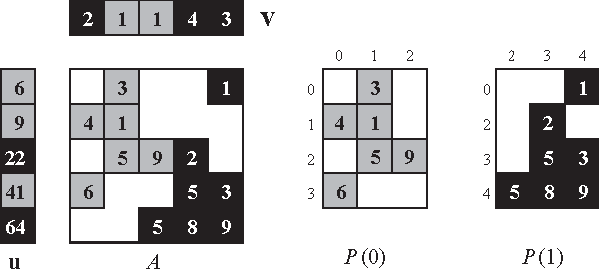
\includegraphics{img/partition}
	\begin{tikzpicture}[scale=0.5]
		\foreach \x / \y in {1/1,1/3,2/2,4/5,4/4,7/3,8/5,6/7,9/1} { \fill[red!90,opacity=.8] ({\y-1},{-\x+1}) rectangle +(1,-1);}
		\foreach \x / \y in {1/2,2/3,3/6,3/9,6/6,5/1,7/8,8/7,9/2} { \fill[blue!60!cyan,opacity=.9] ({\y-1},{-\x+1}) rectangle +(1,-1);}
%		\draw[semithick] (0,-9) grid (9,0);
		\draw[thick] (0,-9) rectangle (9,0);
	\end{tikzpicture}
	\caption{Example of a distribution among two processors of a $9 \times 9$ matrix with 18 nonzeros. Only the sparsity patterns is considered.}
	\label{fig:partition}
\end{figure}

After this distribution, every processor has to compute its local contribution toward the matrix-vector multiplication: to do so, it requires the appropriate vector components which might have been assigned to another processor during the data distribution; if this is the case, communication is required. Once all the required vector components are obtained, the processor starts computing all its local contributions, which are afterwards sent to their appropriate owner, according to the distribution of $u$. The three phases that describe this process for processor $s=0,\dots,p-1$, are summarized in Algorithm \ref{alg:matvec}, from \cite{BSP,mondriaan}.  

\begin{algorithm}[h]
	\begin{algorithmic}
		\Require{$A_s$, the local part of the vector $v$}
		\Ensure{The local part of the vector $u$}
		\State
		\State 	$I_s := \left\{ i | a_{ij} \in A_s \right\}$
		\State 	$J_s := \left\{ j | a_{ij} \in A_s \right\}$
		\State
	\end{algorithmic}
	\begin{enumerate}[(1)]
			\setcounter{enumi}{-1}
		\item 	\begin{algorithmic} \Comment{Fan-out}
				\ForAll{$j \in J_s$}
				\State Get $v_j$ from the processor that owns it. 
				\EndFor
				\State
			\end{algorithmic}
		\item
			\begin{algorithmic} \Comment{Local sparse matrix-vector multiplication}
				\ForAll{$i \in I_s$}
				\State $u_{is} :=0$.
				\ForAll{$j$ such that $a_{ij} \in A_s$}
				\State $u_{is} = u_{is} + a_{ij}v_j$.
				\EndFor
				\EndFor
				\State
			\end{algorithmic}
		\item
			\begin{algorithmic} \Comment{Fan-in}
				\ForAll{$i \in I_s$}
				\State Send $u_{is}$ to the owner of $u_i$.
				\EndFor
				\State
			\end{algorithmic}
	\end{enumerate}
	\label{alg:matvec}
	\caption{Parallel sparse matrix-vector multiplication.}
\end{algorithm}

In reality there is also a fourth phase, in which each processor sums up all the contributions received in phase (2) for all of its owned components of $u$; this is a very small sum with negligible computational cost and for this reason it has been omitted from the algorithm. 

Note that we assume that all of the nonzero values are all represented with the same amount of bits. Doing so, we can focus excusively on the coordinates of the nonzeros, omitting completely their values, as it does not the cost of a parallel sparse matrix-vector multiplication.

Figure \ref{fig:communication} shows an example of the communication involved in supersteps (0) and (2), with the example partitioning shoed in Figure \ref{fig:partition}: the vertical arrows represent the fan out, while the horizontal arrows represent the fan in; the color of an arrow indicates which processor is sending data. 

\begin{figure}[h]
	\centering
	\begin{tikzpicture}[font=\LARGE,scale=0.5]
		\foreach \x / \y in {1/1,1/3,2/2,4/5,4/4,7/3,8/5,6/7,9/1} { \fill[red!90,opacity=.8] ({\y-1},{-\x+1}) rectangle +(1,-1);}
		\foreach \x / \y in {1/2,2/3,3/6,3/9,6/6,5/1,7/8,8/7,9/2} { \fill[blue!60!cyan,opacity=.9] ({\y-1},{-\x+1}) rectangle +(1,-1);}

%		\draw[semithick] (0,-9) grid (9,0);
		\draw[thick] (0,-9) rectangle (9,0);

		\foreach \x in {2,4,5,7} { \fill[red!90,opacity=.8] ({\x-1},4) rectangle +(1,-1);}
		\foreach \x in {1,3,6,8,9} { \fill[blue!60!cyan,opacity=.9] ({\x-1},4) rectangle +(1,-1);}

		\foreach \x in {1,3} { \draw[line width=2pt,blue!60!cyan,opacity=.9,->,>=latex] ({\x-0.5},2.8) -- ({\x-0.5},0.2);}
		\foreach \x in {2,7} { \draw[line width=2pt,red!90,opacity=.8,->,>=latex] ({\x-0.5},2.8) -- ({\x-0.5},0.2);}
%	\draw[->,very thick,>=latex] ({7-0.5},1.8) -- ({7-0.5},{-7+0.2});
%		\draw[semithick] (0,3) grid (9,4);
		\draw[thick] (0,3) rectangle (9,4);

		\foreach \x in {2,4,6,7,9} { \fill[red!90,opacity=.8] (-4,{-\x+1}) rectangle +(1,-1);}
		\foreach \x in {1,3,5,8} { \fill[blue!60!cyan,opacity=.9] (-4,{-\x+1}) rectangle +(1,-1);}

		\foreach \x in {1,8} { \draw[line width=2pt,red!90,opacity=.8,->,>=latex] (-0.2,{-\x+0.5}) -- (-2.8,{-\x+0.5});}
		\foreach \x in {2,6,7,9} { \draw[line width=2pt,blue!60!cyan,opacity=.9,->,>=latex] (-0.2,{-\x+0.5}) -- (-2.8,{-\x+0.5});}
%		\draw[semithick] (-4,-9) grid (-3,0);
		\draw[thick] (-4,-9) rectangle (-3,0);
		\node at (-3.5,-10) {$u$};
		\node at (10,3.5) {$v$};
		\node at (10,-10) {$A$};
	\end{tikzpicture}


%	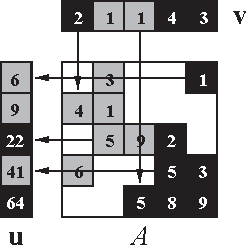
\includegraphics{img/communication}
	\caption{Communication for the sparse parallel matrix-vector multiplication with a matrix partitioned as in Figure \ref{fig:partition}. Vertical arrows represent step (0) while horizontal ones represent step (2). The color of an arrow denotes which processor is sending their data for that row/column.}
	\label{fig:communication}
\end{figure}

As our main interest is to \textbf{minimize} the time spent by the parallel machine computing this sparse matrix-vector multiplication, we need to compute explicitly the cost of Algorithm \ref{alg:matvec}: we can immediately note that such an algorithm, which follows the Bulk Synchronous Parallel model \cite{bsp_paper}, consists of two communication supersteps separated by a computation superstep.

The time spent by a parallel machine in a computation superstep is exactly the time taken by the processor that finishes last: more formally, the time cost of step (1):

\begin{align}
	T_{(1)} = \max_{0 \leq s < p } |A_s|.
	\label{eq:T_comp}
\end{align}

It is easy to understand that, in order to have efficient parallelization, the computation load has to be distributed evenly. Usually, however, it is not possible to achieve a perfect load balance (e.g. when dividing up an odd number of computations among an even number of processors) and we have to reason in terms of an allowed imbalance $\varepsilon$. Consequently, we impose the following hard constraint about the maximum size of the subsets of nonzeros assigned to each processor, according to \cite[eq.~4.27]{BSP}:

\begin{align}
	\max_{0 \leq s <p} |A_s| \leq (1+\varepsilon) \frac{N}{p}.
	\label{eq:balance}
\end{align}

Typical values for the allowed $\varepsilon$ in this constraint are 0.03, i.e. a 3\% imbalance.

It is reasonable, after all, that the problem of finding an efficient way of performing this computation step boils simply down to a hard constraint for the data distribution. This is because we still have to perform all the multiplications of the form $a_{ij} v_j$, no matter our choice. The communication costs, represented by the first and last supersteps in Algorithm \ref{alg:matvec}, are instead the most interesting aspect about maximizing the efficiency of a parallel sparse-matrix vector multiplication algorithm, as there is extreme variability. As a simple example, suppose $p=2$ and consider the matrix represented in Figure \ref{fig:checkered_matrix}. 

\begin{figure}[h]
	\centering
	\begin{tikzpicture}[scale=0.7]
		\draw[thick] (0,0) rectangle (6,-6);
		\foreach \row in {0,1, ..., 5} {
			\foreach \column in {0, ..., 2} {
				\fill[opacity=.8] ({2*\column + mod(\row,2)}, -\row) rectangle +(1,-1);
			}
		};
%		\draw[semithick] (0,-6) grid (6,0);
	\end{tikzpicture}
	\caption{Example matrix with checkered sparsity pattern. Black boxes represent the nonzeros.} \label{fig:checkered_matrix}
\end{figure}

Two possible partitioning of this matrix into two sets are given in Figure \ref{fig:checkered_partitions}. In Figure \ref{fig:checkered_a} no communication is necessary, whereas in Figure \ref{fig:checkered_b}, all of the rows and columns are split, and therefore the maximum possible communication is required during the sparse matrix vector multiplication algorithm.

\begin{figure}[h]
	\centering
	\subfigure[Rows and columns are not split, therefore there is no need for communication.]{
		\begin{tikzpicture}[scale=0.7]
			\foreach \row in {0,2,4} {
				\foreach \column in {0, ..., 2} {
					\fill[opacity=.7,blue] ({2*\column + mod(\row,2)}, -\row) rectangle +(1,-1);
				}
			};
			\foreach \row in {1,3,5} {
				\foreach \column in {0, ..., 2} {
					\fill[opacity=.7,red] ({2*\column + mod(\row,2)}, -\row) rectangle +(1,-1);
				}
			};
%			\draw[semithick] (0,-6) grid (6,0);
			\draw[thick] (0,0) rectangle (6,-6);
		\end{tikzpicture} \label{fig:checkered_a}
	}\hspace{1cm}
	\subfigure[Every row and column is split and causes communication during fan-in and fan-out.]{
		\begin{tikzpicture}[scale=0.7]
			\foreach \index in {0,1, ..., 5} {\fill[opacity=.7,blue] (\index, -\index) rectangle +(1,-1);};
			\foreach \index in {0,1, ..., 3} {\fill[opacity=.7,red] (2+\index, -\index) rectangle +(1,-1);};
			\foreach \index in {0,1, ..., 3} {\fill[opacity=.7,red] (\index, -2-\index) rectangle +(1,-1);};
			\foreach \index in {0,1} {\fill[opacity=.7,blue] (\index, -4-\index) rectangle +(1,-1);};
			\foreach \index in {0,1} {\fill[opacity=.7,blue] (4+\index, -\index) rectangle +(1,-1);};
%			\draw[semithick] (0,-6) grid (6,0);
			\draw[thick] (0,0) rectangle (6,-6);
		\end{tikzpicture} \label{fig:checkered_b}
	}
	\caption{Different partitionings of the matrix from Figure \ref{fig:checkered_matrix}. Red and blue squares represent nonzeros assigned to the two different processors.} \label{fig:checkered_partitions}
\end{figure}

Previously, we claimed that the matrix and both the vectors have to be partitioned: in reality it is sufficient to consider only the problem of distributing the nonzeroes, and the partitioning of the vector can be executed according to this: because of the structure of the communication supersteps in Algorithm \ref{alg:matvec}, we have that communication is required if and only if the rows/columns of the matrices are \emph{cut}, i.e. assigned to more than one processor.

If a full column of our matrix $A$ is assigned to the same processor, we can freely assign the corresponding component of $v$ to the same processor, eliminating completely one source of communication (namely, the fan-out for that column). The same reasoning can be done for the rows. This simplification is possible because imposing a hard constraint similar to \eqref{eq:balance} also to the vector distribution is not very helpful, as it only affects the time of linear vector operations outside the matrix-vector multiplication, which are in generally much cheaper \cite[Sec.~3]{mondriaan}. 

We can describe more formally the communications cost, following the notation of \cite[Def.~2.1]{mondriaan}: let $A_0,\dots,A_{p-1}$ be a $p$-way (with $p \geq 1$) partitioning of the sparse matrix $A$ of size $m \times n$. Let $\lambda_i$ denote the number of processors which have a nonzero of row $i$ and let $\mu_j$ be the number of processors that have a nonzero of column $j$; note that, because we assumed that all the rows and columns are nonempty, we have that $\lambda_i, \mu_j \geq 0$.

Then the total time costs for the communication steps in our Algorithm \ref{alg:matvec} are:

\begin{align}
	\begin{aligned}
		T_{(0)} &= \sum_{j=0}^{n-1} (\mu_j -1), \\
		T_{(2)} &= \sum_{i=0}^{m-1} (\lambda_i -1).
	\end{aligned} \label{eq:T_comm}
\end{align}

These costs are quite straightforward: it is reasonable to assume that the owner of the appropriate vector component is one of the processors that have a nonzero in that row/column, and therefore communication is not necessary. Adding these costs together, we define the \textbf{communication volume} $V$ of the considered partitioning as

\begin{align}
	V := V(A_0,\dots,A_{p-1}) = T_{(0)} + T_{(2)} = \sum_{i=0}^{m-1} (\lambda_i -1) + \sum_{j=0}^{n-1} (\mu_j-1).
	\label{eq:volume}
\end{align}

As we can see, the communication volume $V$ depends entirely on the matrix $A$ and the considered partitioning. Therefore, the problem of minimizing the cost of a matrix-vector multiplication is shifted toward finding an efficient way of distributing the sparse matrix among the available processors, such that our balance constraint \eqref{eq:balance} is satisfied. The following sections and chapters and, ultimately, this whole Master Thesis, are therefore dedicated to it.

\section{Hypergraph model}

The problem of distributing the nonzeros of a matrix in order to minimize the communication volume, or, in short, the matrix partitioning problem, can also be viewed from the graph theory point of view. We recall that a (unweighted, undirected) graph $G=(V,E)$ is a set of vertices (or nodes) $V$ and edges $E$ which connect them. 

The graph partitioning problem has been used in the past to model the load balancing in parallel computing: data are represented as vertices, while their connections (the dependencies) are represented with edges. For a more rigorous definition of the graph partitioning problem, we follow the notation given in \cite{hypergraph_model},  performing the simplification in which all the edges have unitary weight. Given the graph $G=(V,E)$ we say that $(V_0,\dots,V_{p-1})$ is a $p$-way partitioning of $G$ if all these subsets are nonempty, mutually disjoint and their union is the whole set of nodes $V$. 

Moreover, we can consider a balance criterion similar to \eqref{eq:balance}:
\begin{align}
	\max_{0\leq s <p}	|V_s| \leq (1+\varepsilon)\frac{|V|}{p},
	\label{eq:balance_hypergraph}
\end{align}

where $\varepsilon$, similarly as before, represents the allowed imbalance.

Now, given a partition $(V_0,\dots,V_{p-1})$ of the graph $G$, we say that the edge $e=(i,j)$ is \emph{cut} if $i \in V_k, j \in V_l$, with $k \neq l$; otherwise, it is said to be \emph{uncut}. Previously, we claimed that communication during the parallel matrix-vector multiplication can be avoided if a row/column is uncut, and here the goal is the same: we want to minimize the \emph{cutsize}, i.e. the number of edges cut.

However, despite all the similarities between the matrix partitioning problem and the graph partitioning one, it has been shown \cite{hypergraph_model}\cite{zoltan_worth-it},  that this cut-edge metric is not an accurate representation of the communication volume. Additional criticism \cite{hendrickson_emperor} comes from the fact that the graph partitioning approach can only handle square symmetric matrices. It was also shown \cite{hendrickson_kolda} that these disadvantages hold for all application of graph partitioning in parallel computing, and not only our problem of matrix partitioning for sparse matrix-vector multiplication. An exact way of modeling the matrix partitioning problem is through the concept of hypergraph partitioning \cite{hypergraph_model}.

A hypergraph is simply a generalization of a graph: we do not consider edges that connect two nodes, but rather \emph{hyperedges} (or \emph{nets}), which are subsets of nodes. Apart from considering only non-empty hyperedges, note that there is no other restriction on their cardinality.

Hypergraphs, and in particular the hypergraph partitioning problem are already well known in literature: they have a natural application in the designing of integrated circuits (VLSI), in finding efficient storage of large databases on disks, and data mining \cite{vlsi}, as well as urban transportation design and study of propositional logic \cite{papa_hypergraph}.

Because of this extensive application basis, translating our matrix partitioning problem to a hypergraph partitioning problem seems quite convenient, as all the methods already developed can be analyzed and employed also in our case.

Figure \ref{fig:hypergraph} shows an example of such a hypergraph. Each colored set represents a different hyperedge; we can see that we can have hyperedges which contain only one node.

\begin{figure}[h]
	\centering
	%\documentclass{article}
%\pagestyle{empty}
%\usepackage{tikz}

\tikzstyle{vertex} = [fill,shape=circle,node distance=80pt]
\tikzstyle{edge} = [fill,opacity=.5,fill opacity=.5,line cap=round, line join=round, line width=50pt]
\tikzstyle{elabel} =  [fill,shape=circle,node distance=35pt]

\pgfdeclarelayer{background}
\pgfsetlayers{background,main}

%\begin{document}
\begin{tikzpicture}
\node[vertex,label=above:\(v_1\)] (v1) {};
\node[vertex,right of=v1,label=above:\(v_2\)] (v2) {};
\node[vertex,below of=v1,label=above:\(v_4\)] (v4) {};
\node[vertex,right of=v4,label=above:\(v_5\)] (v5) {};
\node[vertex,left of=v4,label=above:\(v_3\)] (v3) {};
\node[vertex,below of=v4,label=above:\(v_7\)] (v7) {};
\node[vertex,left of=v7,label=above:\(v_6\)] (v6) {};

\begin{pgfonlayer}{background}
\draw[edge,color=blue] (v1) -- (v3) -- (v4) -- (v1);
\begin{scope}[transparency group,opacity=.5]
\draw[edge,opacity=1,color=green] (v4) -- (v7);
%\fill[edge,opacity=1,color=green] (v3.center) -- (v5.center) -- (v6.center) -- (v3.center);
\end{scope}
\draw[edge,color=red] (v5) -- (v7);
\draw[edge,color=yellow] (v2) -- (v2);
%\draw[edge,color=blue] (v6) -- (v6);
\end{pgfonlayer}

\node[elabel,color=blue,label=right:{$e_1=\{v_1,v_3,v_4\}$}]  (e1) at (7,0) {};
\node[elabel,below of=e1,color=green,label=right:{$e_2=\{v_4,v_7 \}$}]  (e2) {};
\node[elabel,below of=e2,color=red,label=right:{$e_3=\left\{ v_5,v_7 \right\}$}]  (e3) {};
\node[elabel,below of=e3,color=yellow,label=right:{$e_4=\left\{ v_2 \right\}$}]  (e4) {};
\end{tikzpicture}
%\end{document}
 %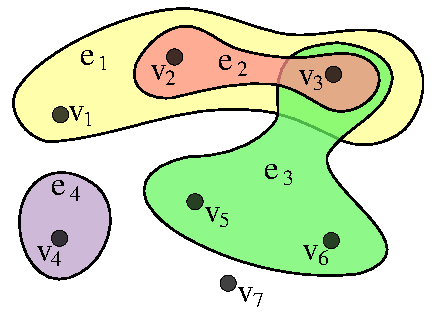
\includegraphics{img/hypergraph}
	\caption{Example of a hypergraph with 7 nodes and 4 hyperedges.}
	\label{fig:hypergraph}
\end{figure}

The definition of hypergraph partitioning problems is identical to the case of a graph, with the difference that now we do not have cut edges, but cut hyperedges: given the hyperedge $e=\{v_1,\dots,v_k\}$, we say that $e$ is cut if there are $i,j$ such that $v_i \in V_r, v_j \in V_s$, with $r \neq s$, i.e. at least two nodes belong to different sets of the partition. As usually, we want to minimize the cut hyperedges.

If, similarly to \eqref{fig:communication}, we define $\lambda_e$ as the number of different sets the vertices in the hyperedge $e$ are assigned to, we have that the total cost of the partition $(V_0,\dots,V_p)$ is:

\begin{align}
	C = C(V_0,\dots,V_{p-1}) = \sum_{e \in E} (\lambda_e -1).
	\label{eq:cost_hypergraph}
\end{align}

We can see how closely these equations resemble the ones given in the previous section: it is clear that the hypergraph partitioning problem closely resembles our original matrix partitioning problem.

Note that the partitioning hypergraph model, along with the simple graph partitioning problem, are known to be NP-hard \cite[Ch.~6]{lengauer}. 

Now, we will describe three possible models for the decomposition of a sparse matrix into a hypergraph, and discuss their advantages and disadvantages.

In the \textbf{column-net} model, our matrix $A$ is represented as a hypergraph for a row-wise decomposition: rows of the matrix are nodes ($V=\{v_1,\dots,v_m\}$, while columns are hyperedges ($E= \{e_1,\dots,e_n\}$). We have that the node $v_i$ belongs to the hyperedge $e_j$ (in short $v_i \in e_j$) if and only if $a_{ij} \neq 0$. With this model, we have that the size of the hyperedge $e_j$ is exactly the number of nonzeros in that column, whereas the node $v_i$ belongs exactly to as many hyperedges as there are nonzeros in that row.

As already said, performing a partitioning on the hypergraph consists of assigning each vertex to one of the sets $V_0,\dots,V_{p-1}$. In this model, this corresponds to assigning a row completely to a processor.However, as vertices are not exactly nonzeros of our matrix, \eqref{eq:balance} and \eqref{eq:balance_hypergraph} are not exactly equivalent; we need to adjust our balance constraint by introducing a weight for each vertex, as in \cite[Def.~4.34]{BSP}. For $v_i \in V$, we define its weight $c_i$ as

\[
	c_i := |\{\;j : \;a_{ij} \neq 0\}|,
\]

which simply is the number of nonzeros in row $i$ of the matrix $A$. Note that, following the same notation as in the previous section, we can see the total number of nonzeros $N$ as $N = \sum_{v_i \in V} c_i$.

Our modified balance constraint is as follows:

\begin{align}
	\max_{0 \leq s <p}	W(V_s) := \max_{0 \leq s <p} \sum_{v_i \in V_s} c_i \leq (1 + \varepsilon) \frac{N}{p}.
	\label{eq:balance_columnet}
\end{align}

The \textbf{row-net} model is very similar to the one just described (as can be guessed from the name): it is exactly the transposed of the colum-net model, in the sense that now rows are hyperedges and columns are vertices of the hypergraph. The reasoning just described applies also to this model, with the little modification that now the weight of a vertex is the number of nonzeros in that column.

We see how the column-net model and row-net model have the advantage of fully assigning a row (or a column) to a processor; this has the advantage of eliminating completely one source of communication in our parallel sparse matrix-vector multiplication algorithm (respectively, the fan-in and fan-out). However, this advantage can easily become a weakness, because now the partitioning is forcedly 1-dimensional, and this is usually too strong of a restriction.

Now, as a last example of possible decomposition of a matrix into a hypergraph, and as a partial address to the drawbacks of the previous two models, we will describe a 2-dimensional approach, the so-called \emph{fine-grain} model \cite{hypergraph_finegrain}. In this model, we have that the $N$ nonzeros are the vertices ($V = \{ v_1,\dots,v_N\}$) and the $m$ rows and $n$ columns are hyperedges ($E = E_r \cup E_c = \{ e_1,\dots,e_m \} \cup \{e_{m+1},\dots,e_{m+n}\}$). With this notation, $E_r$ represents the row hyperedges and $E_c$ represents the column hyperedges. The relationship between the vertices and the hyperedges is fairly obvious: $v_k = a_{ij}$ is in both $e_i$ and $e_{m+j}$.

Now, as the vertices correspond exactly to nonzeros of our matrix, we can use the original equation \eqref{eq:balance_hypergraph} as balance constraint; if we combine this with \eqref{eq:cost_hypergraph}, which describes the cost of a hypergraph partition, we can clearly see how this is identical to our original matrix partitioning problem, described by \eqref{eq:balance} and \eqref{eq:volume}.

On a higher level, one of the benefits of this decomposition model is easy to understand: we have a lot of freedom and we can assign individually each nonzero to a different partition. Similarly as before, however, this advantage can easily become a drawback because now the size of the hypergraph is consistently larger, with $N$ vertices compared to $m$ and $n$ of the previous two models. Thus, computations on the fine-grain model take substantially more time than row-net or column-net models and therefore there is a restriction on the size of the problem that can be efficiently solved.

\section{Earlier work}

Among the models used to translate matrix partitioning into hypergraph partitioning, we already mentioned row-net and column-net \cite{hypergraph_model}, proposed in 1999, and a more recent fine-grained approach \cite{hypergraph_finegrain}, proposed in 2001. New models are relatively rare, and recently Pelt and Bisseling proposed the interesting \textbf{medium-grain} model .  \cite{mediumgrain}.  As this model is at the very base of our work, a more detailed explanation will be given in Section \ref{sec:mediumgrain}.

In addition to these models, there has been some research effort towards the creation of more complicated methods, which often comprise several stages and combine different models.

For example, Uçar and Aykanat \cite{hypergraph_revisiting} first employ an elementary 1-dimensional hypergraph model, and then they transform it in several ways to different hypergraph models suitable for both symmetric and unsymmetric matrix partitionings; it is important to note that these models also include the input and output vectors, and therefore a few extra vertices are added to the hypergraph.

A different 2-dimensional approach is given by the \emph{coarse-grain} method \cite{hypergraph_coarsegrain}: first the column-net hypergraph model is used, obtaining a row partitioning of the matrix in $p$ parts, then a multi-constraint column partitioning in $q$ parts is performed, yielding a final 2-D cartesian partitioning in $p \times q$ parts. 

Moreover, Vastenhouw and Bisseling proposed a 2-dimensional recursive method for data distribution \cite{mondriaan}; this greedy method splits recursively a rectangular matrix into 2 parts.
At each step of the recursion, there is the choice on the direction to be taken in the next step: two different strategies are proposed, alternating splitting directions or simply trying to split both vertically and horizontally and taking greedily the best of the two.

Besides these general purpose models and methods, it is also possible to take into account the structure of the matrix to be partitioned: the hypergraph-based approach was indeed initially devised for structurally symmetric matrices \cite{hypergraph_model}. Moreover, Hu, Maguire and Blake present in \cite{hu2000} an algorithm for nonsymmetric matrices that performs row and column permutations, getting a bordered block diagonal form and then trying to assign matrix rows such that the number of cut columns is minimized.

In general, as there is such a wide variety of different methods and model, it might be difficult to choose the best one, given a matrix to partition. {\c{C}}ataly{\"u}rek, Aykanat, and U{\c{c}}ar propose a partitioning recipe \cite{catalyurek_recipe} that chooses a partitioning method according to some matrix characteristics.

Regarding the actual implementations of the just discussed models, methods and algorithms, there are a few existing software partitioners available. Among the sequential ones we have PaToH (a multilevel Partitioning Tool for Hypergraphs) \cite{patoh}, hMetis \cite{hmetis} (specifically targeted at partitioning hypergraphs for VLSI design), Mondriaan \cite{mondriaan} (among the ones here described, this is the one more specifically designed to solve the matrix partitioning problem), MONET (Matrix Ordering for minimal NET-cut)\cite{hu2000}. Zoltan-PHG (Parallel Hypergraph Partitioner) \cite{parallel_hypergraph} performs instead matrix partitioning in parallel; the relative scarcity of parallel software partitioners is to be explained by the fact that this field is relatively new, and therefore most of the research efforts have been directed toward a sequential approach.

The partitioners just mentioned produce very different results, with respect to both solution quality and execution time, despite having at the core the same method for finding good initial solutions. The method employed is the well-known Kernighan-Lin \cite{kernighan_lin} method, with the optimizations of Fiduccia-Mattheyses \cite{fiduccia}. This local search heuristic was originally designed for bipartitioning graphs and, given a partitioning that obeys the balance constraint \eqref{eq:balance}, it applies a series of small changes to improve the quality of the solution.

To solve large instances, all these partitioners use a multi-level method: the large problem is progressively coarsened until a smaller instance is obtained, then the problem is solved on this small instance and the solution is gradually uncoarsened, with a refinement at each step to improve the solution quality.

Finally, these existing software partitioners are all based on \emph{recursive bisection}: instead of partitioning the hypergraph directly into the desired number of parts, they execute a sequence of bisections of the partitions. This is a good semplification in the sense that it just suffices to find very good algorithms for bipartitioning, and also because splitting a hypergraph in just two parts is much easier; there is however one major flaw with this approach: using this recursive bisection  we might not be able to reach the same quality of a solution with direct splitting into the desired number of parts.

\section{Medium-grain model} \label{sec:mediumgrain}

All of the possible ways of translating the matrix partitioning problem into a hypergraph partitioning problem have different advantages and drawbacks: the 1-dimensional ones, row-net and colum-net, eliminate completely one source of communication but are somewhat too restrictive; fine-grain, on the contrary, does not provide any kind of limitation on the choices for the partitioning, but the resulting hypergraph is very often too big to manage.

A new model has recently been proposed by Pelt and Bisseling \cite{mediumgrain}, which can be described as a sort of middle ground between the 1-dimensional models and fine-grain model. The resulting partitioning is 2-dimensional by design (thus avoiding the limitations of the row-net and column-net models), but it still imposes that clusters of nonzeros from the same rows and columns are assigned to the same processor, thus reducing the size of the final hypergraph, avoiding the main disadvantage of the fine-grain model.

The key of the medium-grain model lies into the splitting of our original matrix $A$ in two parts, $A_r$ and $A_c$, such that $A_r + A_c = A$. Then, we proceed to construct the auxiliary block-matrix $B$, of size $(m+n) \times (m+n)$, defined as

\begin{align}
	B:=	\begin{bmatrix}
		I_n & A_r^T \\
		A_c & I_m
	\end{bmatrix},
	\label{eq:Bmatrix}
\end{align}

where $I_n$ and $I_m$ denote, respectively, the identity matrices of size $n$ and $m$. The final hypergraph is finally obtained by applying the row-net model to this matrix $B$. 

Figure \ref{fig:mediumgrain-1} illustrates this process for a $3 \times 6$ rectangular matrix $A$.

\begin{figure}[h]
	\centering
%	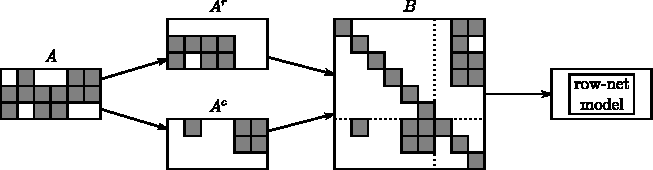
\includegraphics{img/mg-1}
	\begin{tikzpicture}[scale=0.25,font=\large]
	\foreach \x / \y in {1/1,1/3,2/2,4/5,4/4,3/11,4/9,6/7,1/10,2/7} { \fill[purple!90,opacity=.8] ({\y-1},{-\x+1}) rectangle +(1,-1);}
	\foreach \x / \y in {1/2,2/3,3/6,3/9,6/6,5/1,5/12,6/10,2/11,2/8} { \fill[yellow!60!cyan,opacity=.9] ({\y-1},{-\x+1}) rectangle +(1,-1);}
%	\draw[semithick] (0,-6) grid (12,0);
	\draw[thick] (0,-6) rectangle (12,0);
	\node at (6,-7) {$A$};

	\foreach \x / \y in {1/1,1/3,2/2,4/5,4/4,3/11,4/9,6/7,1/10,2/7}{ \fill[purple!90,opacity=.8] ({18+\y-1},{-6-\x+1}) rectangle +(1,-1);}
	\node at (24,-13) {$A_r$};
%	\draw[semithick] (18,{-6-6}) grid ({18+12},-6);
	\draw[thick] (18,{-6-6}) rectangle ({18+12},-6);

	\foreach \x / \y in  {1/2,2/3,3/6,3/9,6/6,5/1,5/12,6/10,2/11,2/8} { \fill[yellow!60!cyan,opacity=.9] ({18+\y-1},{6-\x+1}) rectangle +(1,-1);}
	\node at (24,-1) {$A_c$};
%	\draw[semithick] (18,{-6+6}) grid ({18+12},6);
	\draw[thick] (18,{-6+6}) rectangle ({18+12},6);


	\foreach \x / \y in {1/1,1/3,2/2,4/5,4/4,3/11,4/9,6/7,1/10,2/7}{ \fill[purple!90,opacity=.8] ({36+\y-1},{-6-\x+1}) rectangle +(1,-1);}
	\foreach \x / \y in  {1/2,2/3,3/6,3/9,6/6,5/1,5/12,6/10,2/11,2/8} { \fill[yellow!60!cyan,opacity=.9] ({48+\x-1},{6-\y+1}) rectangle +(1,-1);}


	\foreach \x in {1,2,3,9,10,11} { \fill[gray!10!black,opacity=.9] ({36+\x-1},{6-\x+1}) rectangle +(1,-1);}
	\foreach \x in {1,2,3,6} { \fill[gray!10!black,opacity=.9] ({48+\x-1},{-6-\x+1}) rectangle +(1,-1);}

	% \draw[very thin,help lines] (36,-12) grid (54,6);
	\draw[thick] (36,-12) rectangle (54,6);
	\draw[ultra thick] (48,-12) -- (48,6);
	\draw[ultra thick] (36,-6) -- (54,-6);

	\node at (45,-13) {$B$};

	\draw[line width=1.3pt,>=latex,->] (13,-3) -- (17,-9);
	\draw[line width=1.3pt,>=latex,->] (13,-3) -- (17,3);
	\draw[line width=1.3pt,>=latex,->] (31,-9) -- (35,-4);
	\draw[line width=1.3pt,>=latex,->] (31,3) -- (35,-2);
	
	\draw[line width=1.3pt,>=latex,->] (55,-3) -- (60,-3);
	\node at (64,-2) {row-net};
	\node at (64,-4) {model};
\end{tikzpicture}
\caption{Example of the construction of the matrix $B$ from a $6 \times 12$ matrix $A$, for which the sets $A_r$ and $A_c$ were previously established and colored differently. In the resulting matrix, the dummy nonzeros are depicted in black.}
	\label{fig:mediumgrain-1}
\end{figure}

After we apply the row-net model and obtain a partitioning of the hypergraph, it is immediate to retrieve a partitioning of our matrix $A$, as depicted in Figure \ref{fig:mediumgrain-2}. 

\begin{figure}[h]
	\centering
%	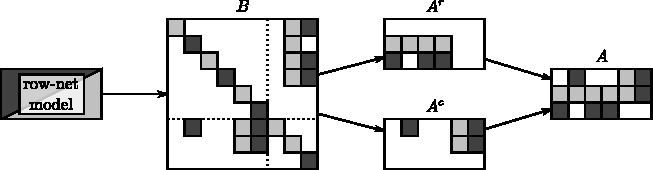
\includegraphics{img/mg-2}
\begin{tikzpicture}[scale=0.25,font=\large]

	\tikzstyle{myred}=[red!90,opacity=.8]
	\tikzstyle{myblue}=[blue!60!cyan,opacity=.9]
	\tikzstyle{myarrow}=[line width=1.3pt,>=latex,->]

	\foreach \x / \y in {1/1,1/3,6/7,1/10,2/7}{ \fill[myred] ({42+\y-1},{-\x+1}) rectangle +(1,-1);}
	\foreach \x / \y in {2/2,4/5,4/4,4/9,3/11}{ \fill[myblue] ({42+\y-1},{-\x+1}) rectangle +(1,-1);}
	\foreach \x / \y in {1/2,2/3,3/6,3/9,6/6,5/1,5/12,6/10,2/11,2/8} { \fill[myred] ({42+\y-1},{-\x+1}) rectangle +(1,-1);}
	\foreach \x / \y in   {2/3,6/6,6/10,2/11,2/8} { \fill[myblue] ({42+\y-1},{-\x+1}) rectangle +(1,-1);}
	%\draw[semithick] (42,-6) grid +(12,6);
	\draw[thick] (42,-6) rectangle +(12,6);

	\node at (48,-7) {$A$};

	\foreach \x / \y in {1/1,1/3,6/7,1/10,2/7}{ \fill[myred] ({24+\y-1},{-6-\x+1}) rectangle +(1,-1);}
	\foreach \x / \y in {2/2,4/5,4/4,4/9,3/11}{ \fill[myblue] ({24+\y-1},{-6-\x+1}) rectangle +(1,-1);}

	\node at (30,-13) {$A_r$};
	%\draw[semithick] (24,{-6-6}) grid +(12,6);
	\draw[thick] (24,{-6-6}) rectangle +(12,6);

	\foreach \x / \y in {1/2,2/3,3/6,3/9,6/6,5/1,5/12,6/10,2/11,2/8} { \fill[myred] ({24+\y-1},{6-\x+1}) rectangle +(1,-1);}
	\foreach \x / \y in   {2/3,6/6,6/10,2/11,2/8} { \fill[myblue] ({24+\y-1},{6-\x+1}) rectangle +(1,-1);}
	\node at (30,-1) {$A_c$};
	%\draw[semithick] (24,{-6+6}) grid +(12,6);
	\draw[thick] (24,{-6+6}) rectangle +(12,6);

	\foreach \x / \y in {1/1,1/3,6/7,1/10,2/7}{ \fill[myred] ({0+\y-1},{-6-\x+1}) rectangle +(1,-1);}
	\foreach \x / \y in {2/2,4/5,4/4,4/9,3/11}{ \fill[myblue] ({0+\y-1},{-6-\x+1}) rectangle +(1,-1);}

	\foreach \x in {1,3,10} { \fill[myred] ({0+\x-1},{6-\x+1}) rectangle +(1,-1);}
	\foreach \x in {2,9,11} { \fill[myblue] ({0+\x-1},{6-\x+1}) rectangle +(1,-1);}


	\foreach \x / \y in  {1/2,2/3,3/6,3/9,6/6,5/1,5/12,6/10,2/11,2/8} { \fill[myred] ({12+\x-1},{6-\y+1}) rectangle +(1,-1);}
	\foreach \x / \y in  {2/3,6/6,6/10,2/11,2/8} { \fill[myblue] ({12+\x-1},{6-\y+1}) rectangle +(1,-1);}


	\foreach \x in {1,3} { \fill[myred] ({12+\x-1},{-6-\x+1}) rectangle +(1,-1);}
	\foreach \x in {2,6} { \fill[myblue] ({12+\x-1},{-6-\x+1}) rectangle +(1,-1);}

	%\draw[very thin,help lines] (0,-12) grid +(18,18);
	\draw[thick] (0,-12) rectangle +(18,18);
	\draw[ultra thick] (12,-12) -- +(0,18);
	\draw[ultra thick] (0,-6) -- +(18,0);

	\node at (9,-13) {$B$};
%
	\draw[myarrow] (19,-3) -- +(4,6);
	\draw[myarrow] (19,-3) -- +(4,-6);
	\draw[myarrow] (37,-9) -- +(4,5);
	\draw[myarrow] (37,3) -- +(4,-5);
%	
	\draw[myarrow] (-6,-3) -- (-1,-3);
	\node at (-10,-2) {row-net};
	\node at (-10,-4) {model};
\end{tikzpicture}

	\caption{Process of obtaining a matrix partitioning starting from a partitioning of the hypergraph following the medium-grain model. In this case $p=2$.}
	\label{fig:mediumgrain-2}
\end{figure}

The usefulness of $A_c$ and $A_r$ is clear if we consider that we use the row-net model. The first is left as-is, while the second is transposed; then, when partitioning 1-dimensionally such that the columns are kept together, we see that we are effectively keeping together elements within the same columns of $A_c$ and $A_r^T$. The resulting partitioning is fully 2-dimensional, because we have clusters of nonzeros: rows for $A_r$ and columns for $A_c$ (hence the subscripts).

The diagonal elements of $B$ are used only to compute the communication volume. Let us consider the $k$th column of $A$; the corresponding nonzeros can be found in the $k$th column of $A_c$  and in the $k$th row of $A_r^T$. If both these parts are nonempty, i.e. the $k$th column of $A$ was not fully assigned to either $A_r$ or $A_c$, we need to be careful when we compute the communication volume of a given partitioning: if these parts are to different processors, communication is needed in Algorithm \ref{alg:matvec}.

Therefore the diagonal nonzero $B_{k,k}$, assigned by the row-net model to the same processor as the $k$th column of $A_c$, that belongs to same row of $B$ as the $k$th row of $A_r$, has the purpose of ensuring a correct computation of the communication volume \cite[Th.~3.1]{mediumgrain}. Note that, implementation-wise, there is no need to have the complete diagonal of $B$: we put a nonzero if and only if the corresponding row of $A_r^T$ and column of $A_c$ are both nonempty.

Experimental results, performed with both the Mondriaan and PaToH packages seems to confirm that this model has indeed some advantages compared to the column-net, row-net and fine-grain models, both regarding partitioning time and solution quality.

Because of these good results, it is our goal to investigate further the properties of this model, following two possible directions.

First of all, as the outcome of the medium-grain model depends remarkably on the initial split of $A$ into $A_r$ and $A_c$, it is interesting to investigate the quality of the algorithm originally proposed in \cite{mondriaan} to achieve this initial partitioning; secondly, we will try to develop a fully iterative method that employs the medium-grain model, where a full multi-level partitioning is performed at each iteration and computation time is traded for solution quality.

Both these research directions share a very important part: we just need to develop efficient methods to compute from the given matrix $A$ the matrices $A_r$ or $A_c$ required for the medium grain model, either from scratch or starting from an already existing partitioning (later in the work we will talk, respectively, about \emph{partition-oblivious} and \emph{partition-aware} algorithms). 

To this extent, Chapters \ref{chap:methods} and \ref{chap:independent_set} describe several of these different methods, whereas in Chapter \ref{chap:experimental_results} we discuss their implementation and the experimental results for the two mentioned research directions.

%\chapter{Strategies for splitting a matrix $A$ into $A_r$ and $A_c$} \label{chap:methods}

The main goal of this thesis is to find efficient ways of splitting our original matrix $A$ into $A_r$ and $A_c$, in order to use the medium-grain model.

We are interested in both improving the initial partitioning of $A$, and a fully iterative method; therefore, we will make the distinction between methods that don't need an initial partitioning (\emph{partition-oblivious} methods), and are therefore suitable for the first case, and methods that do require an initial partitioning (\emph{partition-aware} methods), to be used in a fully iterative scheme. Most of the time the same algorithm can be used for both purposes, albeit with slight modifications.  Before we proceed and analyze the details of the examined heuristics, we can make a few observations, to better understand the general principles behind these algorithms.

If we are interested in an initial partitioning into $A_r$ and $A_c$ that will yield a good communication volume, we already have some information about their quality before the actual partitioning is performed. We can indeed compute an upper bound on the communication cost: if a complete row of $A$ is assigned to $A_r$ (or a full column is assigned to $A_c$), we are sure that those nonzeros will be assigned to the same processor, and we already discussed in Section \ref{sec:par_matvec} how this results in no communication for that row (or column). This can give us the idea of trying to keep, as much as possible, full rows and columns together, although it is impossible to do it all the time (because a given nonzero cannot be assigned to both $A_r$ and $A_c$).

If our purpose is to compute $A_r$ and $A_c$ to improve an existing partitioning, we can follow a few principles to guide us in the choice of what information we should keep, and what we should discard for the next iteration. First of all, it makes sense to have confidence in the existing partitioning: if some nonzeros (for example, a full row or column) are assigned to the same processor, it means that at some point in the previous iteration it was decided that it was convenient to put those nonzeros together, and therefore we should have a preference for them to be together also in the new partitioning. However, this must only serve as an indication and not as a rigid rule, leaving some space for new choices to be made, in order to effectively improve the existing partitioning. Furthermore, we should try to keep, as much as possible, rows and columns together, as noted in the previous paragraph.

\section{Individual assignment of nonzeros} \label{sec:localview}

A simple heuristic that can be used to produce $A_r$ and $A_c$ is a simplification of the algorithm proposed by Pelt and Bisseling along with the medium-grain model \cite[Alg.~1]{mediumgrain}, taking as a \emph{score} function the length (i.e. the number of nonzeros) of the given row or column.

The main idea is to assign each nonzero $a_{ij}$ to $A_r$ if row $i$ is shorter than column $j$ (so it has a higher probability of being uncut in a good partitioning), and to $A_c$ otherwise. Ties are broken, similarly as the original algorithm, in a consistent manner: if the matrix is rectangular we give preference to the shorter dimension, otherwise we perform a random choice.

The partition-oblivious version of this heuristic is given in Algorithm \ref{alg:localview-po}, and it is exactly the same as Algorithm 1 originally proposed. With $nz_r(i)$ we denote the number of nonzeros in row $i$ and with $nz_c(j)$ the number of nonzeros in column $j$.

\begin{algorithm}[h]
	\begin{algorithmic}
		\Require{sparse matrix $A$}
		\Ensure{$A_r$,$A_c$}
		\State
		\If {$m<n$}
		\State $w \gets r$ 
		\ElsIf{$n < m$}
		\State $w \gets c$
		\Else
		\State $w \gets$ random value $c$ or $r$
		\EndIf
		\State $A_r := A_c := \varnothing$
		\ForAll{$a_{ij} \in A$}
		\If{$nz_r(i)<nz_c(j)$}
		\State assign $a_{ij}$ to $A_r$
		\ElsIf{$nz(j)<nz(i)$}
		\State assign $a_{ij}$ to $A_c$
		\Else
		\State assign $a_{ij}$ to $A_w$
		\EndIf
		\EndFor
	\end{algorithmic}
	\caption{Partition-oblivious individual assignment of the nonzeros, based on row/column length.} \label{alg:localview-po}
\end{algorithm}

This algorithm can be easily adapted to compute $A_r$ and $A_c$ from a given partitioning of $A$. Previously we claimed that it is convenient that uncut rows and columns have precedence over cut rows and columns: now, whenever we analyze a nonzero $a_{ij}$ we first look at whether $i$ and $j$ are cut or uncut. If only one of them is cut, we assign the nonzero to the uncut one, otherwise (i.e. both are cut, or both are uncut) we do similarly as before and assign it to the shorter one.

The partition aware variant of this heuristic is given explicitly in Algorithm \ref{alg:localview-pa}.

\begin{algorithm}[h]
	\begin{algorithmic}
		\Require{partitioned sparse matrix $A$}
		\Ensure{$A_r$,$A_c$}
		\State
		\If {$m<n$}
		\State $w \gets r$ 
		\ElsIf{$n < m$}
		\State $w \gets c$
		\Else
		\State $w \gets$ random value $c$ or $r$
		\EndIf
		\State $A_r := A_c := \varnothing$
		\ForAll{$a_{ij} \in A$}
		\If{row $i$ is uncut and column $j$ is cut}
		\State assign $a_{ij}$ to $A_r$
		\ElsIf{row $i$ is cut and column $j$ is uncut}
		\State assign $a_{ij}$ to $A_c$
		\Else
		\If{$nz_r(i)<nz_c(j)$}
		\State assign $a_{ij}$ to $A_r$
		\ElsIf{$nz(j)<nz(i)$}
		\State assign $a_{ij}$ to $A_c$
		\Else
		\State assign $a_{ij}$ to $A_w$
		\EndIf
		\EndIf
		\EndFor
	\end{algorithmic}
	\caption{Partition-aware individual assignment of the nonzeros, based on row/column length.} \label{alg:localview-pa}
\end{algorithm}

In Chapter \ref{chap:experimental_results}, when we are going to perform numerical experiments, we will denote with \verb|po_localview| and \verb|pa_localview|, respectively, the partition-oblivious and the partition-aware variant of this heuristic. 

\section{Assignment of blocks of nonzeros} \label{sec:sbd}

Instead of assigning nonzeros individually as in Section \ref{sec:localview}, we can take a more coarse-grained approach and try to assign at the same time a greater amount of nonzeros to either $A_r$ or $A_c$. In particular, we will discuss how to exploit the Separated Block Diagonal (SBD) form of the partitioned matrix $A$ and introduce a further iteration of this concept, discussing the Separated Block Diagonal of order 2 (SBD2) form of the matrix. Moreover, the heuristics described in this section are all partition-aware, and take as input a partitioned matrix.

As throughout this section the permutations of matrices will be fundamental, we adopt a simplified notation: given a vector $I$ with row indices and a vector $J$ with column indices, we denote as $A(I,J)$ the submatrix of $A$ with only the rows in $I$ and only the columns in $J$ (following the order in which they appear in the vectors). With this notation, for example, $A([1,\dots,m],[1 \dots n]) = A$. Furthermore, if $I_1$ and $I_2$ are both vectors of indices, with $(I_1,I_2)$ we denote the simple concatenation of these vectors.

\subsection{Using the Separated Block Diagonal form of $A$}

The SBD form of a bipartitioned matrix \cite{yzelman_cache} is defined as follows: given a matrix $A$ whose nonzeros are either assigned to processor 0 or 1, we compute the vectors $R_0$ and $R_2$ of the indices of the rows fully assigned, respectively, to processor 0 and processor 1, and the vector $R_1$ of the indices of the rows partially assigned to both of the processors; similarly, we compute $C_0$, $C_2$ and $C_1$ for the columns. Note that, when creating these vectors, their inner ordering is not important; usually, the ascending order is kept.

Then, we obtain the final index vector for the rows as $I = (R_0,R_1,R_2)$ and for the columns as $J = (C_0,C_1,C_2)$. With these quantities, we can finally compute the SBD form of the matrix $A$ as $A(I,J)$. 

An example of the procedure for obtaining this form is shown in Figure \ref{fig:sbd}.

\begin{figure}[h]
	\centering
	\begin{tikzpicture}[scale=0.5]
		\foreach \x / \y in {1/1,1/3,2/2,4/5,4/4,8/5,6/7,9/1} { \fill[myred] ({\y-1},{-\x+1}) rectangle +(1,-1);}
		\foreach \x / \y in {1/2,2/3,3/6,3/9,6/6,5/1,7/8} { \fill[myblue] ({\y-1},{-\x+1}) rectangle +(1,-1);}
%		\draw[help lines] (0,-9) grid (9,0);
		\foreach \x in {0,1,...,8} {\node at ({9.5},{-\x-.5}) {\x};}
		\foreach \x in {0,1,...,8} {\node at ({\x+.5},-9.5) {\x};}


		\foreach \x in {1,2,3} { \fill[mypurple] ({\x-0.5},1) circle (0.4cm);}
		\foreach \x in {4,5,7} { \fill[myred] ({\x-0.5},1) circle (0.4cm);}
		\foreach \x in {6,8,9} { \fill[myblue] ({\x-0.5},1) circle (0.4cm);}

		\foreach \x in {1,2,6} { \fill[mypurple] (-1,{-\x+0.5}) circle (0.4cm);}
		\foreach \x in {4,8,9} { \fill[myred] (-1,{-\x+0.5}) circle (0.4cm);}
		\foreach \x in {3,5,7} { \fill[myblue] (-1,{-\x+0.5}) circle (0.4cm);}

		\draw[very thick] (0,-9) rectangle (9,0);

		\draw[thick,myarrow] (11,-4.5) -- (15,-4.5);
		\node at (12.8,-4) {SBD};
		\foreach \x / \y in {4/4,4/6,5/5,7/8,7/7,8/8,6/9,9/4} { \fill[myred] ({17+\y-1},{-\x+1}) rectangle +(1,-1);}
		\foreach \x / \y in {1/1,1/3,2/4,3/2,4/5,5/6,6/1} { \fill[myblue] ({17+\y-1},{-\x+1}) rectangle +(1,-1);}

%		\draw[help lines] (17,-9) grid ({17+9},0);
		\foreach \x / \y in {2/0,4/1,6/2,0/3,1/4,5/5,3/6,7/7,8/8} {\node at ({17+9.5},{-\y-.5}) {\x};}
		\foreach \x / \y in {5/0,7/1,8/2,0/3,1/4,2/5,3/6,4/7,6/8} {\node at ({17+\y+.5},-9.5) {\x};}


		\foreach \x in {4,5,6} { \fill[mypurple] ({17+\x-0.5},1) circle (0.4cm);}
		\foreach \x in {7,8,9} { \fill[myred] ({17+\x-0.5},1) circle (0.4cm);}
		\foreach \x in {1,2,3} { \fill[myblue] ({17+\x-0.5},1) circle (0.4cm);}

		\foreach \x in {4,5,6} { \fill[mypurple] ({17-1},{-\x+0.5}) circle (0.4cm);}
		\foreach \x in {7,8,9} { \fill[myred] ({17-1},{-\x+0.5}) circle (0.4cm);}
		\foreach \x in {1,2,3} { \fill[myblue] ({17-1},{-\x+0.5}) circle (0.4cm);}

		\draw[very thick] ({17+0},-9) rectangle ({17+9},0);

		\draw[ultra thick] ({17+3},0) -- ({17+3},-9);
		\draw[ultra thick] ({17+6},0) -- ({17+6},-9);

		\draw[ultra thick] ({17+0},-3) -- ({17+9},-3);
		\draw[ultra thick] ({17+0},-6) -- ({17+9},-6);
	\end{tikzpicture}
	\caption{Example process to obtain the SBD form of a partitioned matrix. On the left the original matrix is shown, whereas on the right the permuted SBD form. On the top/left sides of the matrices the color of the circle denotes whether that row/column is completely red or blue or it is mixed (purple), whereas on the bottom/right sides the indices of the columns/rows are explicitly given.} \label{fig:sbd}
\end{figure}

More explicitly, if we denote as $m_i := |R_i|$, $n_i := |C_i|$, with $i=0,1,2$, the SBD form is the resulting block matrix:

\begin{align}\dot{A} := A(I,J) = 
	\begin{bmatrix}
		\dot{A}_{00} & \dot{A}_{01}  & \\
		\dot{A}_{10} & \dot{A}_{11} & \dot{A}_{12} \\
		& \dot{A}_{21} & \dot{A}_{22} \\ 
	\end{bmatrix}, \label{eq:sbd}
\end{align}

where

\begin{itemize}
	\item $\dot{A}_{00}$ of size $m_0 \times n_0$, has nonzeros with uncut rows and uncut columns for processor 0;
	\item $\dot{A}_{22}$ of size $m_2 \times n_2$, has nonzeros with uncut rows and uncut columns for processor 1;
	\item $\dot{A}_{01}$ of size $m_0 \times n_1$, has nonzeros with uncut rows for processor 0 and cut columns;
	\item $\dot{A}_{21}$ of size $m_2 \times n_1$, has nonzeros with uncut rows for processor 1 and cut columns;
	\item $\dot{A}_{10}$ of size $m_1 \times n_0$, has nonzeros with cut rows and uncut columns for processor 0;
	\item $\dot{A}_{12}$ of size $m_1 \times n_2$, has nonzeros with cut rows and uncut columns for processor 1;
	\item $\dot{A}_{11}$ of size $m_1 \times n_1$, has nonzeros with cut rows and columns.
\end{itemize}

Note that the size of each part along with the number of contained nonzeros can greatly vary, also from matrix to matrix: for example, if the sparsity pattern of the matrix allows a ``perfect'' partitioning such that there is no communication, all blocks are empty except $\dot{A}_{00}$ and $\dot{A}_{22}$; conversely, if the matrix has a dense (or complicated) pattern and/or the partitioning is far from optimal, such blocks might be almost empty and $\dot{A}_{11}$ will have the majority of nonzeros. An example of the difference of the block sizes of $\dot{A}$ is shown in Figure \ref{fig:sbd-2}.

\begin{figure}[h]
	\centering
	\subfigure[\texttt{impcol\_b}]{ 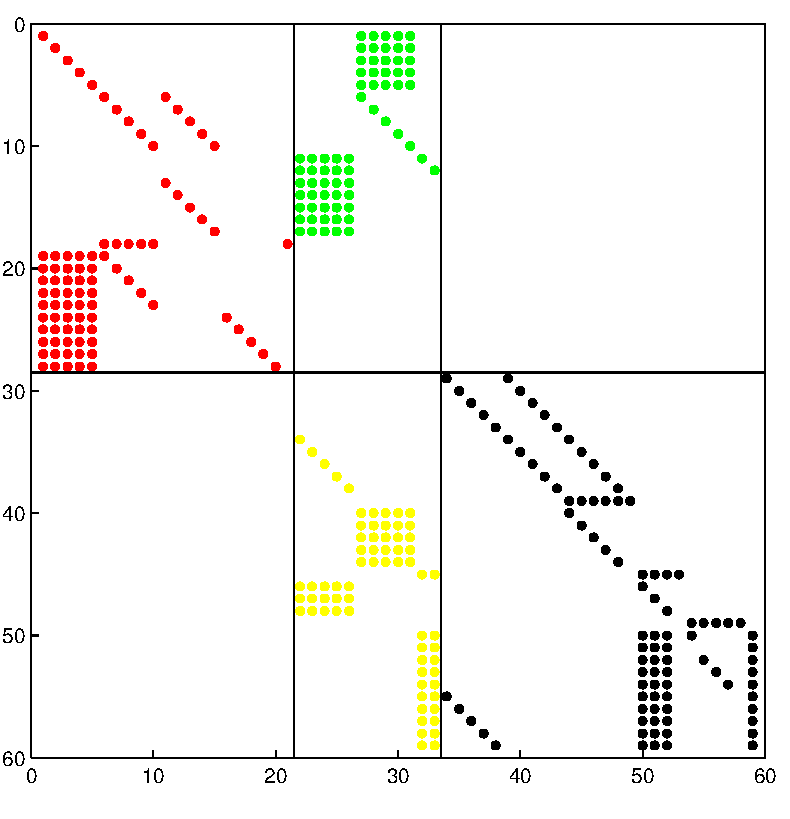
\includegraphics[scale=0.5]{img/impcol_b.pdf} \label{fig:impcol_b}} \hspace{1cm}
	\subfigure[\texttt{cage6}]{ 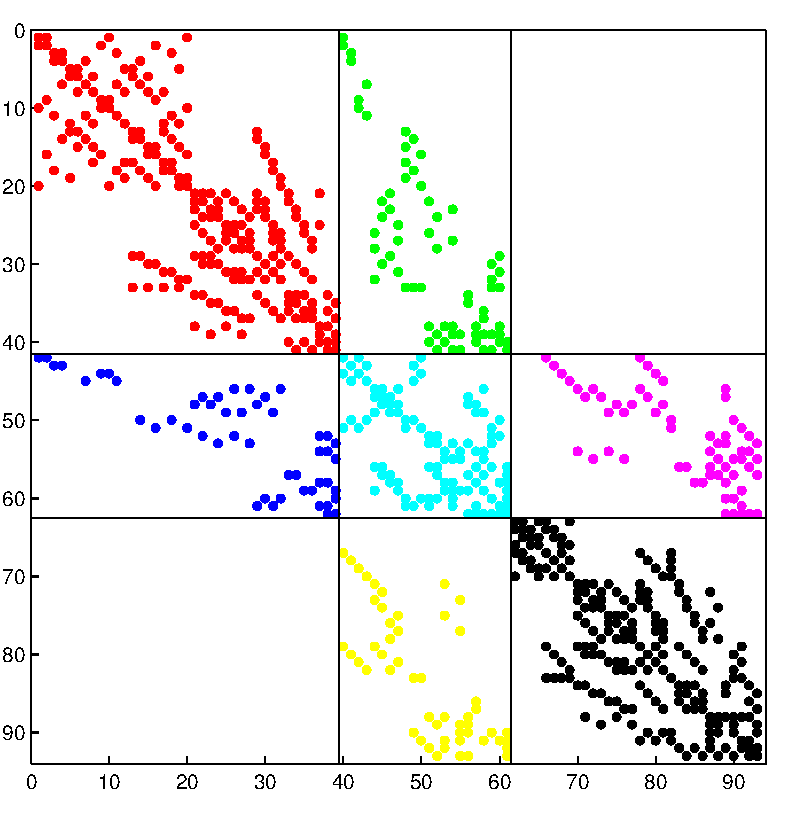
\includegraphics[scale=0.5]{img/cage6.pdf} \label{fig:cage6} }
	\caption{Example of SBD forms of partitioning of the matrices \texttt{impcol\_b} and \texttt{cage6} \cite{ufl}. Each part of $\dot{A}$ has been colored differently. In the first matrix there are no cut rows, which means that $\dot{A}_{10}=\dot{A}_{11} =\dot{A}_{12} = \varnothing$.} \label{fig:sbd-2}
\end{figure}

By computing the Separated Block Diagonal form of a matrix, we are able to explicitly see the underlying structure of the partitioning of a matrix, and the properties of each block can be used to adapt the assignment of its nonzeros. More specifically, the blocks $\dot{A}_{00}$ and $\dot{A}_{22}$ have nonzeros with uncut rows and columns and therefore are more suited to be assigned together; of course, we still have to decide between $A_r$ and $A_c$ and, as mentioned earlier, it is impossible to do both: it is convenient to base our choice on the sizes of such blocks. For example, if $m_0 < n_0$, in the block $\dot{A}_{00}$ the columns are (on average) sparser than the rows: if we assign the nonzeros of this block to $A_c$ we are, in principle, making sure that more rows/columns will stay uncut.

For the blocks with uncut rows and cut columns (namely, $\dot{A}_{01}$ and $\dot{A}_{21}$), the choice is easy: we assign them to $A_r$ and keep their rows uncut. Similarly, we assign the nonzeros of $\dot{A}_{10}$ and $\dot{A}_{12}$ to $A_c$, keeping their columns uncut. 

For the middle block $\dot{A}_{11}$, whose nonzeros have cut rows and cut columns, we cannot exploit any underlying structure: a possible way is to employ one of the other heuristics described in this chapter only considering this submatrix. Our choice is to go with Algorithm \ref{alg:localview-po} presented in Section \ref{sec:localview} (note that we cannot exploit the partition-aware variant of it, because all of the nonzeros in the block considered have cut rows and columns).

The heuristic that employs the SBD structure of a matrix can be explictly visualized in \eqref{eq:sbdview}.

\begin{align}
	\text{	Assignment of } \dot{A}:	\begin{bmatrix}
		R/C & R & \\
		C & M & C \\
		& R & R/C \\
	\end{bmatrix}
	\label{eq:sbdview}
\end{align}

In this matrix, whose structure is the same of \eqref{eq:sbd}, the letter $R$ in a block denotes that we assign that block to $A_r$, and similarly for $C$ and $A_c$. Moreover, $R/C$ stands that the choice between $A_r$ and $A_c$ depends on the block size, whereas $M$ indicates that the block is assigned in a mixed manner, according to Algorithm \ref{alg:localview-po}.

Note that, as mentioned in Chapter \ref{chap:introduction}, the matrix is usually split by means of recursive bipartitionings: it is then sufficient to keep track of the order of these recursions to have an implicit ordering which can be easily used to compute the SBD form of a matrix \cite{yzelman_cache}, instead of computing this form from scratch using the algorithm described in \cite[Appendix A]{bas}.

In Chapter \ref{chap:experimental_results}, we will refer to the algorithm described in this section as \verb|pa_sbdview|.

\subsection{Using the Separated Block Diagonal form of order 2 of $A$} \label{sec:sbd2}

The proposed SBD2 form of a partitioned matrix $A$ is an extension of the SBD form: given a partitioned matrix $A$, we compute the Separate Block Diagonal form of $A$ of order 2 by separating, in $\dot{A}_{10}$ and $\dot{A}_{12}$ the empty and non-empty columns, and in $\dot{A}_{01}$ and $\dot{A}_{21}$ the empty and non-empty rows. Then all the other blocks, except the central one, are permuted and split up accordingly. This procedure is better shown in Algorithm \ref{alg:sbd2}. 

\begin{algorithm}[h]
	\begin{algorithmic}
		\Require{ partitioned matrix $A$}
		\Ensure{$\ddot{A}$}
		\State compute $\dot{A}$ as the SBD form of $A$ and obtain also $R_0,R_1,R_2,C_0,C_1,C_2$;
		\State split $R_0$ in $R_{00}$ and $R_{01}$, such that $A(R_{00},C_1) = \varnothing$;
		\State split $R_2$ in $R_{20}$ and $R_{21}$, such that $A(R_{21},C_1) = \varnothing$;
		\State split $C_0$ in $C_{00}$ and $C_{01}$, such that $A(R_1,C_{00}) = \varnothing$;
		\State split $C_2$ in $C_{20}$ and $C_{21}$, such that $A(R_1,C_{21}) = \varnothing$;
		\State $I:= (R_{00},R_{01},R_1,R_{20},R_{21})$;
		\State $J:= (C_{00},C_{01},C_1,C_{20},C_{21})$;
		\State $\ddot{A} := A(I,J)$.
	\end{algorithmic}
	\caption{Algorithm to obtain SBD2 form of a matrix $A$.} \label{alg:sbd2}
\end{algorithm} 

The resulting final matrix is a block tridiagonal matrix $\ddot{A}$:

\begin{align}
	\ddot{A} := \begin{bmatrix}
		\ddot{A}_{00} & \ddot{A}_{01} & & & \\
		\ddot{A}_{10} & \ddot{A}_{11} & \ddot{A}_{12} & & \\
		& \ddot{A}_{21} & \ddot{A}_{22} & \ddot{A}_{23} & \\
		& & \ddot{A}_{32} & \ddot{A}_{33} & \ddot{A}_{34} \\
		& & & \ddot{A}_{43} & \ddot{A}_{44} \\
	\end{bmatrix},
	\label{eq:sbd2}
\end{align}

where each submatrix $\ddot{A}_{pq}$ is of size $m_p \times n_q$.

Figure \ref{fig:sbd2} shows the process of obtaining this matrix $\ddot{A}$ starting from the SBD matrix $\dot{A}$ obtained in Figure \ref{fig:sbd}.

\begin{figure}[h]
	\centering
	\begin{tikzpicture}[scale=0.5]
		\foreach \x / \y in {4/4,4/6,5/5,7/8,7/7,8/8,6/9,9/4} { \fill[myred] ({0+\y-1},{-\x+1}) rectangle +(1,-1);}
		\foreach \x / \y in {1/1,1/3,2/4,3/2,4/5,5/6,6/1} { \fill[myblue] ({0+\y-1},{-\x+1}) rectangle +(1,-1);}

%		\draw[help lines] (0,-9) grid ({0+9},0);
		\foreach \x / \y in {2/0,4/1,6/2,0/3,1/4,5/5,3/6,7/7,8/8} {\node at ({0+9.5},{-\y-.5}) {\x};}
		\foreach \x / \y in {5/0,7/1,8/2,0/3,1/4,2/5,3/6,4/7,6/8} {\node at ({0+\y+.5},-9.5) {\x};}

		\node at (1.5,-10.7) {$C_0$};
		\node at (4.5,-10.7) {$C_1$};
		\node at (7.5,-10.7) {$C_2$};

		\node at (11,-1.5) {$R_0$};
		\node at (11,-4.5) {$R_1$};
		\node at (11,-7.5) {$R_2$};

		\draw[very thick] ({0+0},-9) rectangle ({0+9},0);

		\draw[ultra thick] ({0+3},0) -- ({0+3},-9);
		\draw[ultra thick] ({0+6},0) -- ({0+6},-9);

		\draw[ultra thick] ({0+0},-3) -- ({0+9},-3);
		\draw[ultra thick] ({0+0},-6) -- ({0+9},-6);

		\draw[thick,myarrow] (13,-4.5) -- (17,-4.5);

		\foreach \x / \y in {4/4,4/6,5/5,8/9,8/8,9/9,6/7,7/4} { \fill[myred] ({19+\y-1},{-\x+1}) rectangle +(1,-1);}
		\foreach \x / \y in {1/3,1/2,3/4,2/1,4/5,5/6,6/3} { \fill[myblue] ({19+\y-1},{-\x+1}) rectangle +(1,-1);}

%		\draw[help lines] (19,-9) grid ({19+9},0);
		\foreach \x / \y in {2/0,6/1,4/2,0/3,1/4,5/5,8/6,3/7,7/8} {\node at ({19+9.5},{-\y-.5}) {\x};}
		\foreach \x / \y in {7/0,8/1,5/2,0/3,1/4,2/5,6/6,3/7,4/8} {\node at ({19+\y+.5},-9.5) {\x};}

		\node at ({19+1},-10.7) {$C_{00}$};
		\node at ({19+2.5},-10.7) {$C_{01}$};
		\node at ({19+4.5},-10.7) {$C_{1}$};
		\node at ({19+6.5},-10.7) {$C_{20}$};
		\node at ({19+8},-10.7) {$C_{21}$};

		\node at ({19+11},-1) {$R_{00}$};
		\node at ({19+11},-2.5) {$R_{01}$};
		\node at ({19+11},-4.5) {$R_{1}$};
		\node at ({19+11},-6.5) {$R_{20}$};
		\node at ({19+11},-8) {$R_{21}$};

		\draw[very thick] ({19+0},-9) rectangle ({19+9},0);

		\draw[ultra thick] ({19+3},0) -- ({19+3},-9);
		\draw[ultra thick] ({19+6},0) -- ({19+6},-9);
		\draw[ultra thick] ({19+2},0) -- ({19+2},-9);
		\draw[ultra thick] ({19+7},0) -- ({19+7},-9);

		\draw[ultra thick] ({19+0},-3) -- ({19+9},-3);
		\draw[ultra thick] ({19+0},-6) -- ({19+9},-6);
		\draw[ultra thick] ({19+0},-2) -- ({19+9},-2);
		\draw[ultra thick] ({19+0},-7) -- ({19+9},-7);
	\end{tikzpicture}
	\caption{SBD2 form obtained starting from the SBD form of Figure \ref{fig:sbd}.} \label{fig:sbd2}
\end{figure}

To better understand the interesting properties of the newly created parts of the matrix, let us introduce the concept of \emph{neighbor}: given the nonzero $a_{ij}$ we say that $a_{kl}$ is a neighbor if $k = i \vee l = j$; in other words, neighbors of a given nonzero are the ones that lie in the same row or in the same column.

Now, let us consider, for sake of brevity, just the top-left corner of $\ddot{A}$: nonzeros in $\ddot{A}_{00}$ are uncut in the rows and columns and whose neighbors are uncut also in the other, non-shared, dimension. Similarly, nonzeros in $\ddot{A}_{01}$ do not have any neighbor (w.r.t. their row) with cut columns but have neighbors (w.r.t their column) with cut rows. And similarly, with the roles of rows and columns reversed, for $\ddot{A}_{10}$. This exact same reasoning applies also for the bottom-right corner, with the appropriate adaptation of indices.

The size of these parts, and more generally of all of the blocks of $\ddot{A}$, is again highly dependent on the structure of the matrix, as shown in Figure \ref{fig:sbd2-2}.

\begin{figure}[h]
	\centering
	\subfigure[\texttt{impcol\_b}]{ 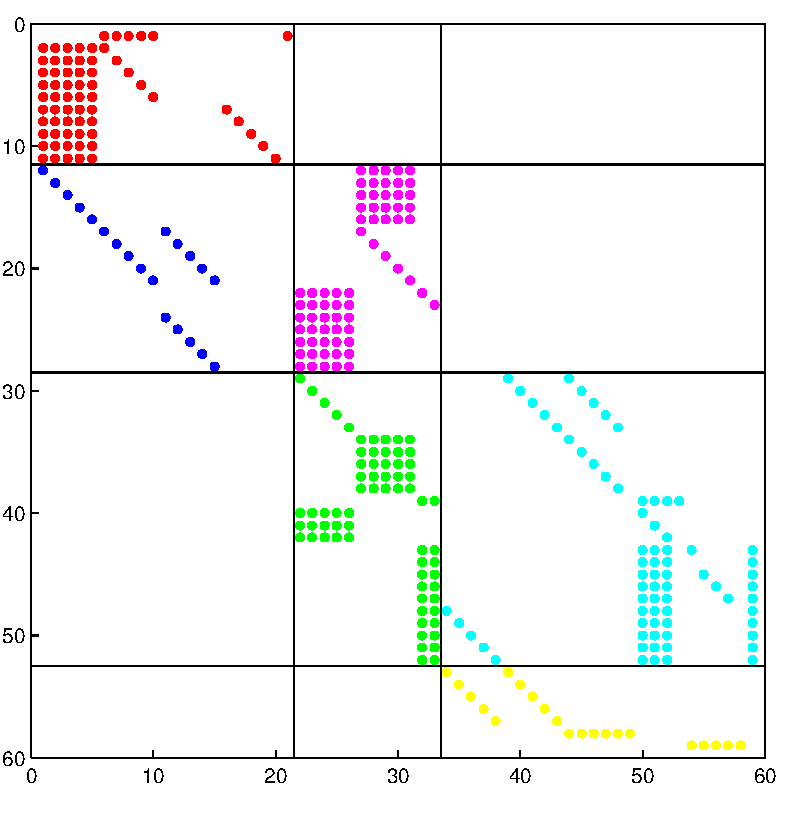
\includegraphics[scale=0.5]{img/sbd2_impcol_b.pdf} \label{fig:sbd2_impcol_b}}\hspace{1cm} 
	\subfigure[\texttt{cage6}]{ 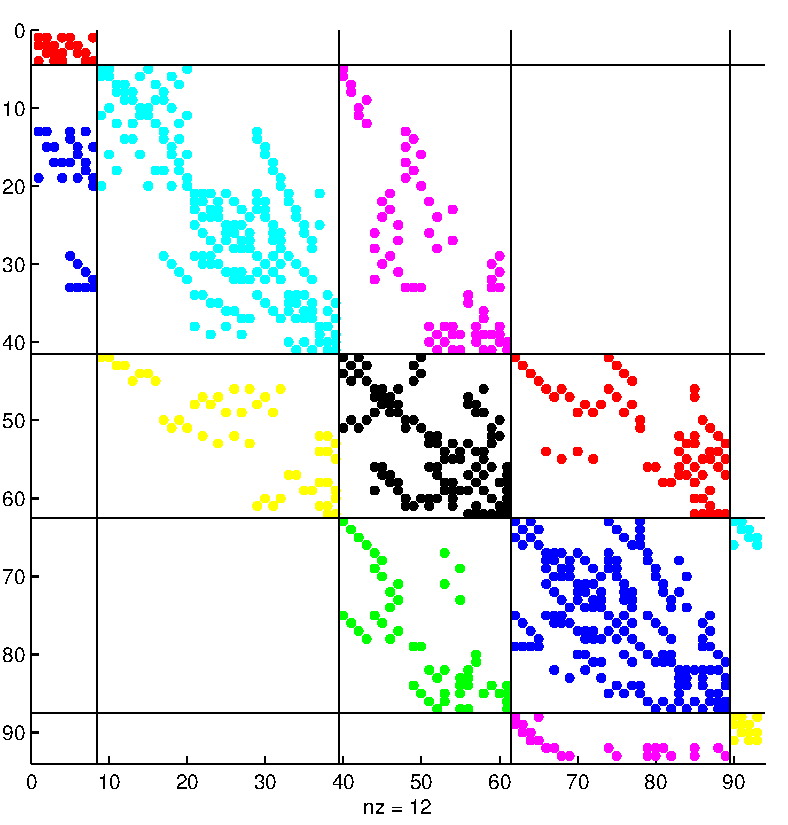
\includegraphics[scale=0.5]{img/sbd2_cage6.pdf} \label{fig:sbd2_cage6} }
	\subfigure[\texttt{sherman1}]{ 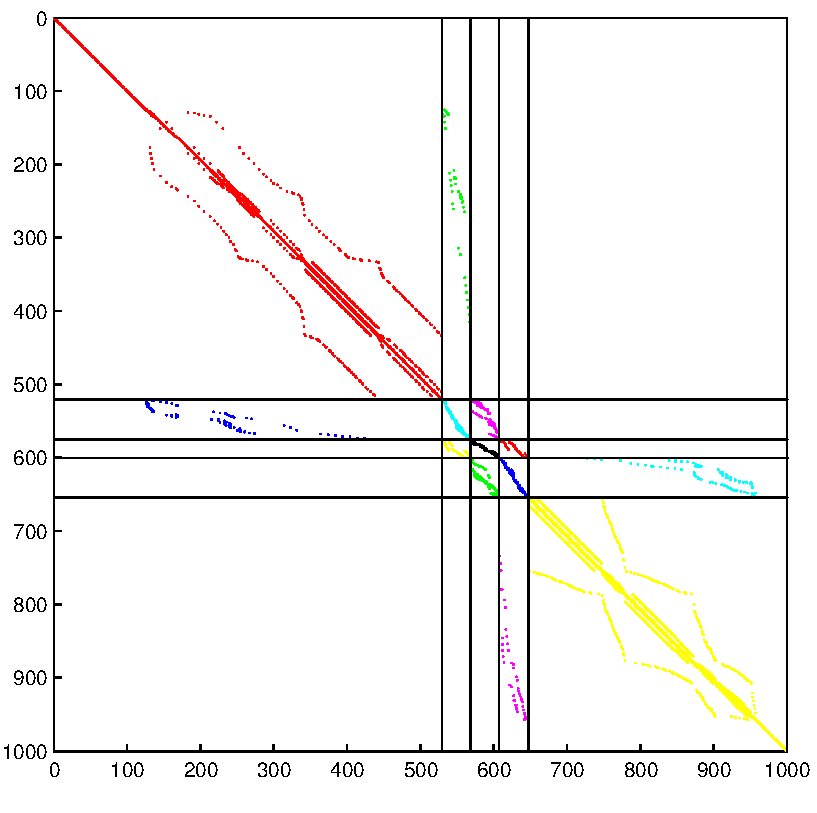
\includegraphics[scale=0.5]{img/sbd2_sherman1.pdf} \label{fig:sbd2_sherman1}} 
	\caption{Example of SBD2 forms of three different matrices. Similarly as in Figure \ref{fig:sbd-2}, each part of $\ddot{A}$ has been given a color (note that since there are more parts than coloris used, some colors are repeated even though the parts are not related in any way).	We can see in \ref{fig:sbd2_impcol_b} that the second and fourth columns are empty, and therefore not shown in the image. We can also see the difference in structure between \ref{fig:sbd2_cage6} and \ref{fig:sbd2_sherman1}: the former one comes from a DNA electrophoresis problem \cite{ufl}, while the latter is an oil reservoir simulation challenge matrix \cite{matrixmarket}. We can see that with the \texttt{sherman1} matrix, the corner parts are predominant because it is a finite element matrix, with a strongly diagonal pattern: it makes sense that most of these nonzeros are ``independent'' from each other. }  \label{fig:sbd2-2}
\end{figure}

Other than the corner blocks, for which we already argued that the matrix partitioning problem is easy, this structure enables us to assign more specifically nonzeros to either $A_r$ or $A_c$: it is convenient to assign $\ddot{A}_{01}$ and $\ddot{A}_{43}$ to $A_r$, as these nonzeros can be fully assigned to one processor without having the columns cut, and similarly we can assign $\ddot{A}_{10}$ and $\ddot{A}_{34}$ to $A_c$; for the other blocks, we can repeat the reasoning of the last section.

This heuristic that exploits the SBD2 form of the matrix $A$ is given explicitly as follows:

\begin{align}
	\text{Assignment of } \ddot{A}: \begin{bmatrix}
		R & R & & & \\
		C & R/C & R & & \\
		& C & M & C & \\
		& & R & R/C & C \\
		& & & R & C \\
	\end{bmatrix}
	\label{eq:sbd2view}
\end{align}

$R$ denotes, as previously, that the block as been assigned to $A_r$ and similarly for $C$ and $A_c$. $R/C$ denotes that the assignment depends on the block size and $M$ that a mixed assignment is performed with Algorithm \ref{alg:localview-po}.

Note that, in this case, the SBD2 form has to be computed from scratch from the SBD form, because it uses further information that is not employed during the normal partitioning.

In Chapter \ref{chap:experimental_results}, we will refer to the algorithm described in this section as \verb|pa_sbd2view|.

\section{Maximizing empty rows of $B$} \label{sec:globalview}

In this section, instead of describing a generating scheme that takes as input the matrix $A$ and produces as output $A_r$ and $A_c$, we will introduce an improvement scheme, which operates on already existing $A_r$ and $A_c$ and tries to refine them such that the upper bound on the communication volume is lowered.

At the beginning of this chapter, we mentioned how it is convenient to have full rows assigned to $A_r$ and full columns assigned to $A_c$, in order to avoid communication; a good strategy to produce good $A_r$ and $A_c$, could then be to maximize such full assignments. The proposed heuristic does essentially this, by trying to swap the assignment of nonzeros from $A_r$ to $A_c$ and viceversa, trying to obtain that full rows are assigned to $A_r$ and full columns are assigned to $A_c$. In order to achieve both of these goals with a unique algorithm, it is convenient to reason in terms of the matrix $B$ as in \eqref{eq:Bmatrix}. If we maximize the number of empty rows of $B$, we are effectively emptying rows of $A_r^T$ (i.e. emptying columns of $A_r$, therefore fully assigning nonzeros in them to $A_c$) and of $A_c$, thus assigning full rows to $A_r$.

This improvement heuristic falls into the category of \emph{local search} algorithms: we start from a configuration (an assignment of nonzeros to $A_r$ and $A_c$) and perform a search on the neighborhood, defined as the set of configurations which differ only by the assignment of a single nonzero. By performing this small swap, we can easily fall in a local optimum situation: a few nonzeros (depending on the structure of the matrix) are continuously swapped between $A_r$ and $A_c$. 

We can add a little hill-climbing capability to our heuristic by adding a little buffer: we pre-determine $l_{max}$, the maximum amount of worsening allowed, and, after this threshold is reached, we start considering only strictly improving solution. In order to have a meaningful threshold, it might be convenient to have it relative to the amount of rows/columns of $B$, or to its nonzeros. The higher this threshold is, the more capability we have of escaping local optima, but at the cost of slowing down considerably the improvement (even potentially arresting it) of our solution.

For the choice of the neighbor configuration to consider, it is convenient to consider the row of $B$ with a diagonal element (which corresponds to a split row/column of $A$) with the minimum number of nonzeros: our immediate goal, which in reality spans over a few moves of our local search, is to fully assign the nonzeros of this row of $B$; we consider the minimum because each time we swap we might slightly worsen the solution.

A more explicit overview on this local search improvement scheme is described in Algorithm \ref{alg:globalview}:

\begin{algorithm}[h]
	\begin{algorithmic}
		\Require{$A_r$, $A_c$, $l_{max}$, $iter_{max}$}
		\Ensure{$A_r'$, $A_c'$}
		\State $l := 0$
		\State Compute $B$ following the medium-grain model
		\For{$it=1,\dots,iter_{max}$}
		\State $\displaystyle i := \argmin_{k \in \{1,\dots,m+n\}\text{ s.t. }B(k,k) \neq 0} nz_r(k)$
		\ForAll{$j \neq i$ such that $B(i,j) \neq 0$}
		\If{$B(j,j) \neq 0$} 
		\State $B(i,j) = 0$
		\State $B(j,i) = 1$
		\Else
		\If{$l < l_{max}$}
		\State $B(i,j) = 0$
		\State $B(j,i) = 1$
		\State $l = l+1$
		\EndIf
		\EndIf
		\EndFor
		\If{$nz(B(i)) = 1$}
		\State $B(i,i) = 0$
		\State $l = l-1$
		\EndIf
		\EndFor
		\State $A_r' := B([1,\dots,n],[n+1,\dots,m+n])^T$
		\State $A_c' := B([n+1,\dots,m+n],[1,\dots,n])$	
	\end{algorithmic}
	\caption{Local search refinement of $A_r$ and $A_c$} \label{alg:globalview}
\end{algorithm}

As this is a scheme that relies on existing $A_r$ and $A_c$ and aims at improving them, we still need to choose how to generate these parts in the first place. If we can rely on an existing partitioning, a simple choice could be to take as $A_r$ and $A_c$ the subsets of nonzeros assigned, respectively, to processor 0 and 1; otherwise, if our goal is to produce $A_r$ and $A_c$ for the initial partitioning, the simplest choice is to randomly assign each nonzero to either $A_r$ or $A_c$. These initial solutions, however, are fast to generate but not particularly efficient, and are therefore meaningful only if our improvement scheme is fast enough; otherwise, we can always rely on one of the other heuristics described in this chapter.

\section{Partial assignment of rows and columns} \label{sec:hot_restart}

In Section \ref{sec:localview} we discussed how to assign each nonzero independently, whereas in Section \ref{sec:sbd} we examined the possibility of exploiting a little the structure of the matrix, in order to assign more nonzeros at once. Keeping this direction, there is some other structure of $A$ that can lead to a better assignment: partial assignment of rows and columns.

The main idea behind this heuristic is that, every time we assign a nonzero to $A_r$, we know that it is convenient that also all the other nonzeros in the same row are assigned to it; conversely, if a nonzero is assigned to $A_c$, all the nonzeros in its column should stick with it. Therefore, we ideally want to keep together rows and columns as much as possible; but, as already discussed, there is always the problem that a nonzero cannot be assigned to both $A_r$ and $A_c$, we can only reason in term of partial assigment of the row/column. 

Throughout this section we will stop distinguishing between rows and columns of a matrix and reason in term of \textbf{indices} in the set $\{0,\dots,m+n-1\}$: following the natural ordering, the $m$ rows are mapped to $0,\dots,m-1$ and the $n$ columns to $m,\dots,m+n-1$.

This simplification of terms is due to the fact that the core of this heuristic lies in the computation of a \textbf{priority vector} $v$, which is none other than a permutation of the indices $0,\dots,m+n-1$, where they appear in order of decreasing priority: in this sense, the priority is to be intended as the probability of the nonzeros of that index to be together in a good partitioning.

The assignment of nonzeros is done by ``painting'' them with an imaginary color, which corresponds either to $A_r$ or $A_c$: we iterate through our priority vector backwards (i.e. starting from the index with the lowest priority) and assign all of its nonzeros to go together: if the index corresponds to a row, then we assign all of its nonzeros to $A_r$, otherwise we assign them to $A_c$. Because each nonzero has both a row and a column, it is represented twice in our priority vector; the second time it is considered, we re-assign it by ``painting it over'' (hence the name of the algorithm).

A more explicit formulation of this procedure is given in Algorithm \ref{alg:overpainting}.

\begin{algorithm}[h]
	\begin{algorithmic}
		\Require{Priority vector $v$, matrix $A$}
		\Ensure{$A_r$, $A_c$}
		\State $A_r := A_c: = \varnothing$
		\For{$i=m+n-1,\dots,0$}
		\If{$v_i < m$}
		\State Add the nonzeros of row $i$ to $A_r$
		\Else
		\State Add the nonzeros of column $i$ to $A_c$
		\EndIf
		\EndFor
	\end{algorithmic}
	\caption{Overpainting algorithm} \label{alg:overpainting}
\end{algorithm}

It is possible also to give an alternative formulation for this algorithm in which we iterate forward through $v$, as described in Algorithm \ref{alg:overpainting-2}.

\begin{algorithm}[h]
	\begin{algorithmic}
		\Require{Priority vector $v$, matrix $A$}
		\Ensure{$A_r$, $A_c$}
		\State $A_r := A_c: = \varnothing$
		\For{$i=0,\dots,m+n-1$}
		\If{$v_i < m$}
		\State Add the unmarked nonzeros of the row $i$ of $A$ to $A_r$
		\Else
		\State Add the unmarked nonzeros of the column $i$ of $A$ to $A_c$
		\EndIf
		\State Mark nonzeros of index $i$ as ``evaluated''
		\EndFor
	\end{algorithmic}
	\caption{Alternative formulation of Algorithm \ref{alg:overpainting}.} \label{alg:overpainting-2}
\end{algorithm}

In this formulation, every assignment to $A_r$ and $A_c$ is final, but with the added complexity of checking which nonzeros of the considered index are still to be assigned, and only work with them.

Lastly, another different formulation is possible: we consider individually each nonzero $a_{ij}$ and see whether in $v$ $i < j$ (where the $<$ symbol is to be intended as ``$i$ precedes $j$'' and not as the comparison of the values) or the other way around; in the first case, the row has more priority and we assign $a_{ij}$ to $A_r$, otherwise we assign it to $A_c$. Note that, since we have to perform $N$ lookups on the vector $v$, this is a more expensive formulation of the same algorithm.

An important point to observe is that this overpainting algorithm is completely deterministic: $A_r$ and $A_c$ are uniquely determined by the ordering of the indices in $v$. Therefore, the heuristic part of this algorithm lies entirely in the choice of this priority vector, and, for this reason, we will focus on it in the next subsection. 

\subsection{Computation of the priority vector $v$}

Because, with the overpainting algorithm, the quality of $A_r$ and $A_c$ depends entirely on the choice of $v$, it is important to take a structured approach and explore a wide variety of possibilities for this priority vector.

In this section, we proceed and define several \emph{generating schemes}, and their input determines whether the overpainting algorithm is used to obtain a better initial partitioning or a fully iterative scheme. In general, we try to come up with schemes that can be used for either purpose, with slight modifications. 

Each one of the generating schemes can be summarized in three main steps:

\begin{enumerate}
	\item usage of previous partitioning;
	\item sorting;
	\item internal ordering of indices.
\end{enumerate}

Now, we give a more detailed explanation of each of those steps. 

\begin{itemize}
	\item \textbf{usage of previous partitioning}: if we are considering \emph{partition aware generating schemes}, we separate the set of uncut indices (i.e. indices which correspond to uncut rows or columns) from the  cut indices. We consider the simple concatenation of uncut indices and cut indices, in this order, and the next steps are performed on each of these parts. If, instead, we are considering a \emph{partition oblivious scheme}, the subsequent operations are performed on the set $\{0,\dots,m+n-1\}$.

	\item \textbf{sorting}: we can either keep the set from the previous step untouched (therefore preserving the natural order of indices) or perform a sorting with respect to the number of nonzeros. The sorting is done in ascending order, as a short row/column is more likely to fit completely in a good partitioning because it does not yield many cut columns/rows.

		In addition, we can refine a bit our sorting: we could move the indices which have only one nonzero to the back, because no matter our assignment of such nonzero, that index will not be cut and it is best to try to keep also the other dimension uncut. 

	\item \textbf{internal ordering}: as the last step, we want to finalize our vector $v$ by deciding more precisely the position of each index. The strategies considered, which often depend internally on an additional parameter, are the following:

		\begin{itemize}
			\item \textbf{concatenation}: we put either all the rows before all the columns, or all the columns before all the rows;
			\item \textbf{mixing}: we can mix rows and columns in two main ways: alternation and spread. Suppose there are twice as many columns as rows: in the first case we get
				$$(c,r,c,r,c,r,\dots,c,r,c,c,c,\dots,c,c,c),$$

				whereas with the second one we get 

				$$(c,c,r,c,c,r,\dots,c,c,r),$$

				where with $c$ we denote a generic column and with $r$ a generic row. To obtain a more even distribution, we always start with the greater dimension.
			\item \textbf{random} (only in case of no sorting): we randomize the ordering of the indices;
			\item \textbf{simple} (only in case of sorting): we let the sorting decide completely the ordering, and the vector is left as is.
		\end{itemize}
\end{itemize}

As the complete description of a generating scheme is somewhat lengthy, we use a simplified notation and adopt the following abbreviations:

\begin{itemize}
	\item \verb|PO|: partition oblivious
	\item \verb|PA|: partition aware
	\item \verb|sorted| and \verb|unsorted|: sorting w.r.t. the number of nonzeros is performed or not
	\item \verb|w| and \verb|nw|: all the indices with only 1 nonzero are moved to the back or not
	\item \verb|simple|: the sorted vector is left as-is
	\item \verb|concat|: rows and columns are concatenated
	\item \verb|row|: the concatenation is done rows-columns
	\item \verb|col|: the concatenation is done columns-rows
	\item \verb|mix|: mixing of the rows and columns is enforced
	\item \verb|alt|: rows and columns are alternated
	\item \verb|spr|: rows and columns are spread
	\item \verb|random|: the order of the indices is randomized
\end{itemize}

With this notation, the name \verb|po_sorted_nw_mix_spr| stands for ``partition oblivious generating scheme, with indices sorted by number of nonzeros, without moving the indices with 1 nonzero to the back, with forced mixing of rows and columns, in a spread fashion''. This is just one of the many possibilities, which are convenient to visualize using a directed graph, as shown in Figure \ref{fig:digraph}; a generating scheme is simply a path from START to END. 

\begin{figure}[h]
	\begin{center}
		\begin{tikzpicture}[every path/.style={>=latex}]
			\node (start) at (6,14) {START};
			\node (po) at (4.5,12.5)  { PO };
			\node (pa) at (7.5,12.5) { PA };
			\node (d1) at (6,11.5) {$\bullet$};
			\node (sorted) at (3,9.5) {sorted};
			\node (unsorted) at (10.5,9.5) {unsorted};
			\node (w) at (2,8.25) {w};
			\node (nw) at (4,8.25) {nw};
			\node (d3pre) at (3,7) {$\bullet$};
			\node (d3) at (6,5) {$\bullet$};
			\node (concat) at (4.5,3) {concat}; 
			\node (mix) at (7,3) {mix};
			\node (random) at (10.5,3) {random};
			\node (simple) at (1,3) {simple};
			\node (alt) at (6.5,2) {alt};
			\node (row) at (4,2) {row};
			\node (col) at (5,2) {col};
			\node (end) at (6,-0.5) {END};
			\node (spr) at (7.5,2) {spr};

			\draw[->] (start) edge (po);
			\draw[->] (start) edge (pa);

			\draw[->] (po) edge (d1);
			\draw[->] (pa) edge (d1);

			\draw[->] (d1) edge (sorted);
			\draw[->] (d1) edge (unsorted);

			\draw[->] (sorted) edge (w);
			\draw[->] (sorted) edge (nw);

			\draw[->] (unsorted) edge (d3);
			\draw[->] (w) edge (d3pre);
			\draw[->] (nw) edge (d3pre);
			\draw[->] (d3pre) edge (d3);
			\draw[->] (d3pre) edge (simple);

			\draw[->] (d3) edge (mix);
			\draw[->] (d3) edge (concat);

			\draw[->] (unsorted) edge (random);

			\draw[->] (mix) edge (alt);
			\draw[->] (mix) edge (spr);

			\draw[->] (alt) edge (end);
			\draw[->] (spr) edge (end);

			\draw[->] (concat) edge (row);
			\draw[->] (concat) edge (col);

			\draw[->] (row) edge (end);
			\draw[->] (col) edge (end);
			\draw[->] (simple) edge (end);
			\draw[->] (random) edge (end);

			\draw[dashed] (0,13.25) -- (13,13.25);
			\draw[dashed] (0,10.5) -- (13,10.5);
			\draw[dashed] (0,4) -- (13,4);
			\draw[dashed] (0,0.5) -- (13,0.5);

			\node[align=left,draw] at (13,12) {usage of previous \\partitioning};
			\node[align=left,draw] at (13,7) {sorting};
			\node[align=left,draw] at (13,2) {internal ordering};
		\end{tikzpicture}
	\end{center}
	\caption{Directed graph that represents the family of heuristics used (any path from START to END). Dummy nodes (the ones without any label) were added in order to reduce the number of edges and ease legibility.} \label{fig:digraph}
\end{figure}

Other than this family of heuristics, we can also formulate the problem of partial assignment of rows/columns, always following this framework, in another more mathematical way, to which we dedicate Chapter \ref{chap:independent_set}.

%\chapter{Independent set formulation of the partial row/column assignment problem} \label{chap:independent_set}

With the framework introduced in Section \ref{sec:hot_restart}, we basically translated the problem of the assignment of nonzeros to $A_r$ and $A_c$ (which is already another formulation of the matrix partitioning problem with the medium grain model) to the problem of an efficient computation of a permutation of the indices $0,\dots,m+n-1$. In this chapter, we will propose a method for this vector computation problem, which relies on concepts of the field of graph theory.

The main idea is somewhat similar to the principle that lead us to the development of the Separated Block Diagonal form of order 2 in Section \ref{sec:sbd2}. In that particular form of a partitioned matrix, as already argued, the blocks $\ddot{A}_{00}$ and $\ddot{A}_{44}$ are interesting, because they contain nonzeros with the property of being ``independent''. More precisely, those were rows and columns fully assigned to a processor and whose nonzeros didn't have any neighbor (a nonzero in the same row or column) which had a cut column/row. These nonzeros, then, could be assigned anywhere that they still did not cause communication.

The term \emph{independent}, in this reasoning, has to be defined very carefully: we want to look for a subset of $\{0,\dots,m+n-1\}$ which does not any communication, whenever we fully assign its rows to $A_r$ and its columns to $A_c$. With this definition, our goal is clear: we want to assign as much nonzeros as possible in this way, lowering consistently the upper bound on the communication volume that can be computed during the creation of $A_r$ and $A_c$.

To do so, we can employ a very well studied object in graph theory: the \textbf{independent set}. However, this requires a correct translation of our sparse matrix into a graph, in order to produce the desired result, which is described in Section \ref{sec:is_graph}. In Section \ref{sec:is_comp}, instead, we discuss the actual algorithm used to compute the maximum independent set in such graph.

\section{Graph construction} \label{sec:is_graph}

In order to retrieve the desired information from the graph, we need to construct it correctly from our sparse matrix. In our case, we can simply consider the graph whose adjacency matrix is none other than the sparsity pattern of our matrix $A$. This exact same formulation has already been studied for the matrix partitioning problem, under the name of \emph{bipartite graph model} by Hendrickson and Kolda \cite{hendrickson}, where the authors, after constructing the graph, discuss different algorithms for bipartite graph partitioning and come to the conclusion that the best strategy is using multilevel methods with Fiduccia-Mattheyses refinement.

More specifically, in this graph formulation we have that rows and columns are vertices, and we have the edge $(i,j)$ if $a_{ij} \neq 0$; the resulting graph is bipartite.

An example of such translation from matrix to graph is shown in Figure \ref{fig:bipartite_graph}, where we translate the matrix given in Figure \ref{fig:partition}. 

\begin{figure}[h]
	\centering
	\begin{tikzpicture}[scale=0.5]
		\tikzstyle{myred}=[red!90,opacity=.8]
		\tikzstyle{myblue}=[blue!60!cyan,opacity=.9]
		\tikzstyle{mypurple}=[purple!80!blue,opacity=.9]
		\tikzstyle{myarrow}=[line width=1.3pt,>=latex,->]
		\tikzstyle{vertex} = [fill,shape=circle,node distance=100pt,minimum size=0.2cm,inner sep = 0pt]
		\foreach \x / \y in {1/1,1/3,2/2,4/5,4/4,7/3,8/5,6/7,9/1} { \fill[myred] ({\y-1},{-\x+1}) rectangle +(1,-1);}
		\foreach \x / \y in {1/2,2/3,3/6,3/9,6/6,5/1,7/8,8/7,9/2} { \fill[myblue] ({\y-1},{-\x+1}) rectangle +(1,-1);}
%		\draw[semithick] (0,-9) grid (9,0);
		\draw[thick] (0,-9) rectangle (9,0);

		\draw[myarrow,thick] (10,-4.5) -- (13,-4.5);

		\foreach \x in {0,...,8} { 
			\node[vertex,label=left:\(r_{\x}\)] (r\x) at (16,{3.5-2*\x}) {}; 
			\node[vertex,label=right:\(c_{\x}\)] (c\x) at (26,{3.5-2*\x}) {};
			\node at (-1,{-\x-0.5}) {\x};
			\node at (\x+0.5,1) {\x};
		}


			\foreach \x / \y in {0/0,0/2,1/1,3/4,3/3,6/2,7/4,5/6,8/0} { \draw[myred] (r\x) -- (c\y);}
			\foreach \x / \y in {0/1,1/2,2/5,2/8,5/5,4/0,6/7,7/6,8/1} { \draw[myblue] (r\x) -- (c\y);} 
		\end{tikzpicture}
		\caption{Graph constructed using the sparsity pattern of the matrix of Figure \ref{fig:partition} as adjacency matrix (rows and columns are vertices, nonzeros are edges). The edge color is the same of the corresponding nonzeros, but only to facilitate the understanding of this translation; in reality there is no distinction between edges. With $r_i$ we denote row $i$, whereas with $c_j$ we denote column $j$.} \label{fig:bipartite_graph}
	\end{figure}


\section{Computation of the independent set} \label{sec:is_comp}
\subsection{Hopcroft-Karp algorithm} \label{sec:hopcroft}


%\chapter{Implementation and experimental results} \label{chap:experimental_results}

In Chapter \ref{chap:methods} and \ref{chap:independent_set} we discussed different heuristics aimed at solving the the matrix partitioning problem; whether we try to improve the initial partitioning or perform a fully iterative procedure, we need to translate those ideas into practice, devising an efficient implementation.

In Section \ref{sec:earlier_work}, we mentioned existing software partitioners: Mondriaan \cite{mondriaan} is the package of our choice and we defer to it the actual computations of the partitionings, limiting ourselves to create the matrix $B$ of the medium-grain model as in \eqref{eq:Bmatrix}. The actual algorithm used to construct this matrix is given explicitly in Algorithm \ref{alg:B}. Note how we consider only the sparsity patterns of $A$, neglecting completely the values of the nonzeros.

\begin{algorithm}[h]
	\begin{algorithmic}
		\Require{$A_r$, $A_c$}
		\Ensure{$B$}
		\State $B \gets \varnothing$
		\ForAll{$a_{ij} \in A_c$} \Comment{The part relative to $A_c$}
		\State $b_{i+n,j} = 1$
		\EndFor
		\ForAll{$a_{ij} \in A_r$} \Comment{The part relative to $A_r$}
		\State $b_{j,i+n} = 1$
		\EndFor
		\For{$j=1,\dots,n$} \Comment{Dummy nonzeros for cut columns}
		\If{$\exists\, i$ s.t. $a_{ij} \in A_r$ and $\exists\, i'$ s.t. $a_{i'j} \in A_c$}
		\State $b_{j,j} = 1$
		\EndIf
		\EndFor
		\For{$i=1,\dots,m$} \Comment{Dummy nonzeros for cut rows}
		\If{$\exists\, j$ s.t. $a_{ij} \in A_r$ and $\exists\, j'$ s.t. $a_{ij'} \in A_c$}
		\State $b_{n+i,n+i} = 1$
		\EndIf
		\EndFor
	\end{algorithmic}
	\caption{Construction of $B$ following the medium-grain model.} \label{alg:B}
\end{algorithm}

Now, having discussed the means of obtaining $A_r$ and $A_c$ and the matrix $B$, we can outline the general framework used to test the effectiveness of the proposed heuristics. The framework is given explicitly in Algorithm \ref{alg:framework}, and it takes as a parameter the maximum number of iterations allowed, $iter_{max}$.  

\begin{algorithm}[h]
	\begin{algorithmic}
		\Require{Sparse matrix $A$}
		\Ensure{Partitioning for the matrix $A$}
		\State Partition $A$ with Mondriaan using the default options and the medium-grain method
		\For{$i=1,\dots,iter_{max}$}
		\State Use any of the heuristics described previously to compute $A_r$ and $A_c$
		\State construct $B$, using Algorithm \ref{alg:B}, from $A_r$ and $A_c$
		\State Partition $B$ with Mondriaan using the default options and the row-net model
		\State Re-construct $A$ with the new partitioning
		\EndFor
	\end{algorithmic}
	\caption{General framework for the testing of our heuristics} \label{alg:framework}
\end{algorithm}

In Chapter \ref{chap:methods} and \ref{chap:independent_set}, we distinguished between partition-oblivious and partition-aware methods, and Algorithm \ref{alg:framework} is suitable for both types of heuristics: even though the framework is naturally suited for developing a fully iterative scheme, if we desire a better initial partitioning for the medium-grain method, we can simply neglect the partitioning done in the first step. This is precisely the scope of a partition-oblivious heuristic.

Regarding the actual implementation, we can see from Algorithm \ref{alg:framework} that Mondriaan is used to perform the actual partitioning and this is the ideal case for its use as a software library. As a consequence, we used C as the main implementation language, even though MATLAB was used for faster prototyping: the flexibility added by managing objects at runtime  is ideal when designing algorithms. In order to have C code and MATLAB code interact in the correct way, we took advantage of MEX files \cite{mex}. In general, unless preliminary tests showed that the considered heuristic had a remarkably bad quality, we translated back most of the programs to the C language, in order to remove the MEX layer of complexity and get a more efficient implementation. For the Hopcroft-Karp algorithm described in Chapter \ref{chap:independent_set}, we used an implementation \cite{hkarp_impl} written in the Python programming language, which computes directly the matching on a bipartite graph and the maximum independent set. 

In order to perform effective numerical experiments, we need to have a consistent way of testing. First of all, since we seek heuristics suitable for many matrices, it makes sense to have several matrices to test for, as described in Section \ref{sec:test_matrices}. 

Secondly, since randomness is involved in the partitioner itself and, to a different extent, in some of the heuristics, we need to take several measurements and compute an average. After generating an initial partitioning, one iteration of the heuristic was performed independently 5 times, and their result was averaged; this was repeated 20 times, obtaining an average of the 20 initial partitioning and an average of the 20 averages of final results. 

Lastly, in order to have a meaningful result that can help us understand whether the given heuristic is globally effective, we will compute the geometric mean of all the initial partitioning and the geometric mean of all the final results. Then, we will normalize w.r.t the first value. Doing so, we can understand whether the considered heuristic performs better or worse in a consistent way. This normalized geometric mean is denoted, in the following tables, with the symbol $\rho$.

\section{Test matrices} \label{sec:test_matrices}

In order to have insightful results, we mentioned that the matrices used in the numerical experiments should have different features: in particular we distinguish between rectangular matrices and square matrices, and try to have a wide selection w.r.t. the number of nonzeros. 

These matrices are mainly from the University of Florida Sparse Matrix Collection \cite{ufl}, and some can additionally be found on the Matrix Market collection \cite{matrixmarket}. The matrices \verb|tbdmatlab| and \verb|tbdlinux| are from \cite{mondriaan}. Table \ref{tab:matrices} provides a more thorough description of the matrices used, along with an outline of their basic properties (number of rows $m$, number of columns $n$, number of nonzeros $N$) and their original purpose. Some of these matrices (namely the ones with the $\dagger$ symbol in the table) belong to the 10th Dimacs Implementation Challenge \cite{dimacs}, which addressed the graph partitioning and graph clustering problem, and are therefore naturally suited for testing the quality of the solutions produced by our algorithms. The three symmetric matrices which represent street networks, are the undirected and unweighted version of the largest strongly connected component of the corresponding OpenStreetMap road network of that country.

\begin{table}[h]
	\centering
	\begin{tabular}{|l|r|r|r|p{7cm} |}
		\hline	
		\textbf{Name} & \textbf{$m$} & \textbf{$n$} & \textbf{$N$} & \textbf{Source problem} \\ \hline
		\verb|lpi_ceria3d| 									& 3576 		& 4400 		& 21178 & Netlib Linear Programming \\
		\verb|dfl001| 											& 12230 	& 6071 		& 35632 & Netlib Linear Programming \\ 
		\verb|delaunay_n15| $\dagger$ 			& 32768 	& 32768 	& 196548 & Delaunay triangulations of random points in plane \\ 
		\verb|deltaX| 											& 68600 	& 21961 	& 247424 & High fillin with exact partial pivoting \\
		\verb|cre_b| 												& 9648 		& 77137 	& 260785 & Netlib Linear Programming \\ 
		\verb|tbdmatlab| 										& 19859 	& 5979 		& 430171 & Term-by-document matrix \\ 
		\verb|nug30|												& 52260 	& 379350 	& 1567800 & Netlib Linear Programming \\ 
		\verb|coAuthorsCiteseer| $\dagger$ 	& 227320 	& 227320 	& 1628268 & Citation and coauthor network\\ 
		\verb|bcsstk32| $\dagger$ 					& 44609 	& 44609 	& 2014701 & Stiffness matrix for automobile chassis \\ 
		\verb|bcsstk30| $\dagger$						& 28924 	& 28924 	& 2043492 & Stiffness matrix for off-shore generator platform \\
		\verb|wave| 	$\dagger$							& 156317 	& 156317 	& 2118662 & 3D finite elements \\
		\verb|tbdlinux| 										& 112757 	& 20167 	& 2157675 & Term-by-document matrix \\
		\verb|rgg_n_2_18_s0| $\dagger$ 			& 262144 	& 262144 	& 3094566 & Random graph \\
		\verb|belgium_osm| $\dagger$				& 1441295 & 1441295 & 3099940 & Street network of Belgium\\
		\verb|polyDFT| 											& 46176 	& 46176 	& 3690048 & Polymer self-assembly \\ 
		\verb|netherlands_osm| $\dagger$		& 2216688 & 2216688 & 4882476 & Street network of The Netherlands \\
		\verb|cage13| 											& 445315 	& 445315 	& 7479343 & DNA Electrophoresis \\
		\verb|italy_osm| $\dagger$					& 6686493 & 6686493 & 14027956 & Street network of Italy\\
		\hline
	\end{tabular}
	\caption{Matrices used in our experiments, sorted by number of nonzeros.} \label{tab:matrices}
\end{table}

In Figures \ref{fig:patterns1}, \ref{fig:patterns2} and \ref{fig:patterns3}, we show the sparsity patterns of the test matrices. The images were obtained using the \verb|spy| function of MATLAB.

%\begin{figure}[h]
%	\centering
%	\subfigure[\texttt{lpi\_ceria3d}]{ 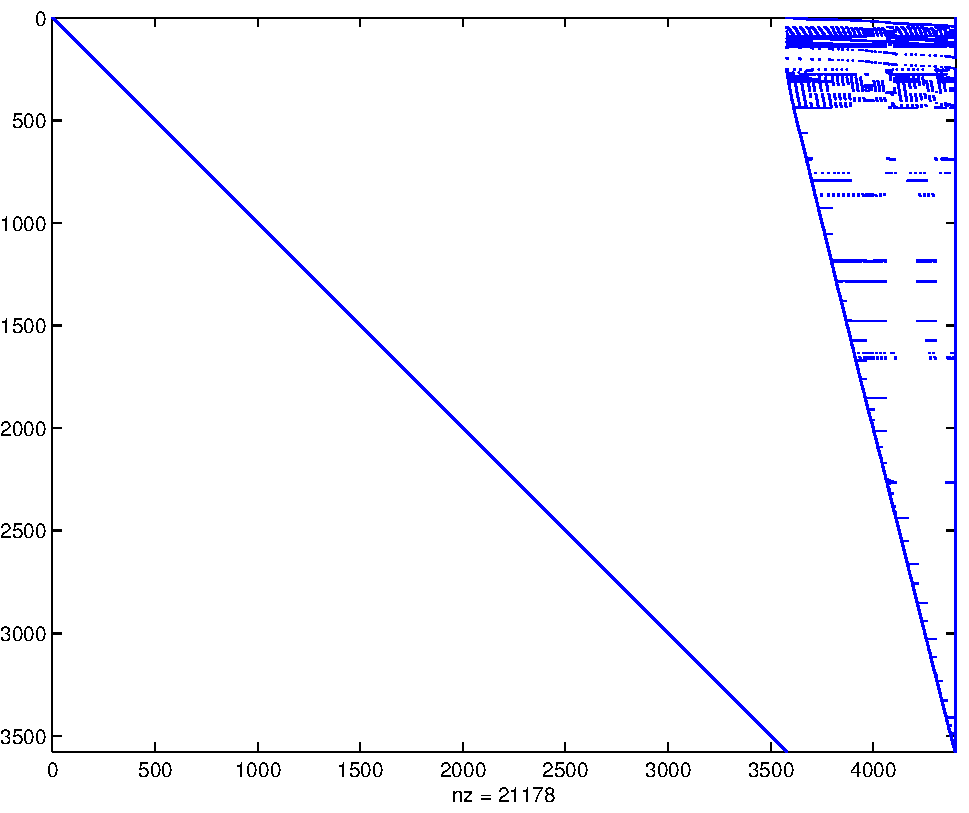
\includegraphics[scale=0.45]{img/lpi_ceria3d.pdf} \label{fig:lpi_ceria3d}}
%	\subfigure[\texttt{dfl001}]{ 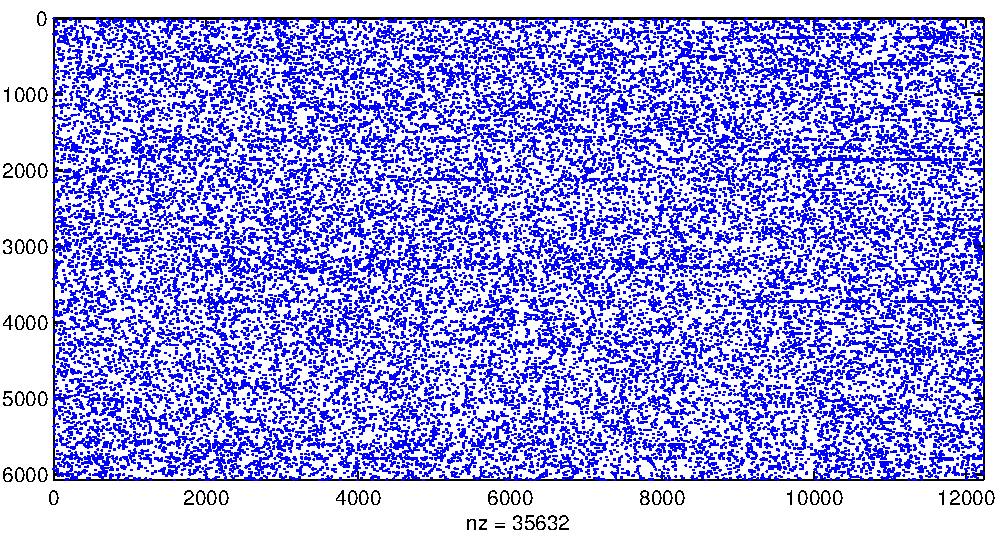
\includegraphics[scale=0.45]{img/dfl001.pdf} }
%	
%	\subfigure[\texttt{delaunay\_n15}]{ 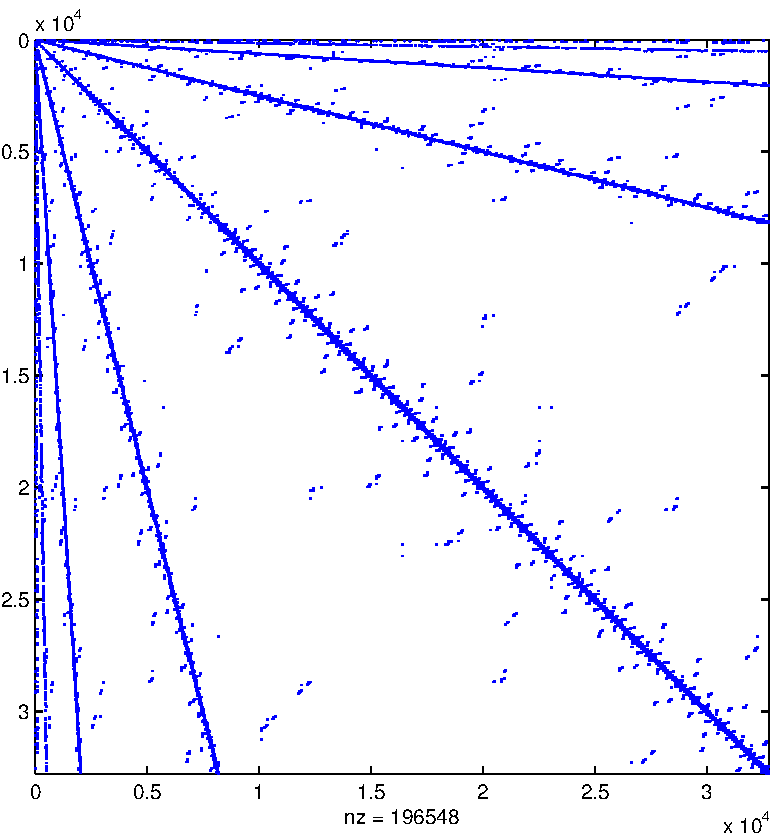
\includegraphics[scale=0.45]{img/delaunay_n15.pdf} }
%	\subfigure[\texttt{deltaX}]{ 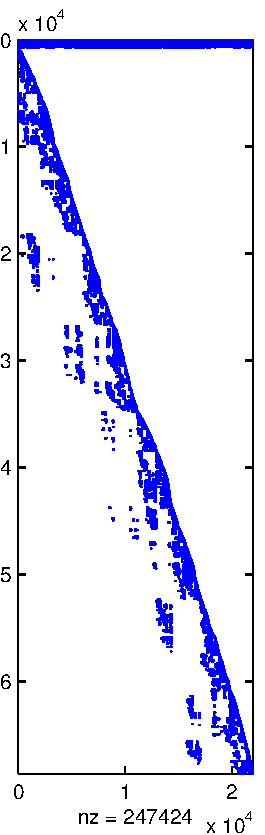
\includegraphics[scale=0.45]{img/deltaX.pdf} }
%	
%	\subfigure[\texttt{cre\_b}]{ 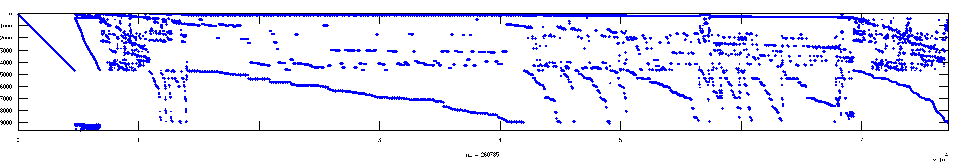
\includegraphics[scale=0.45]{img/cre_b.pdf} }
%	\subfigure[\texttt{tbdmatlab}]{ 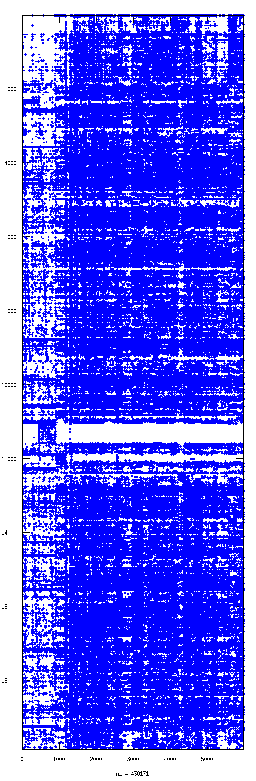
\includegraphics[scale=0.45]{img/tbdmatlab.pdf} }
%	\caption{Sparsity patterns of the test matrices.} \label{fig:patterns1}
%\end{figure}
%
%\begin{figure}[h]
%	\centering
%	\subfigure[\texttt{nug30}]{ 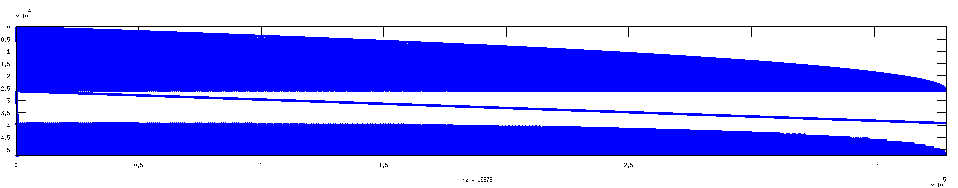
\includegraphics[scale=0.45]{img/nug30.pdf} }
%	\subfigure[\texttt{coAuthorsCiteseer}]{ 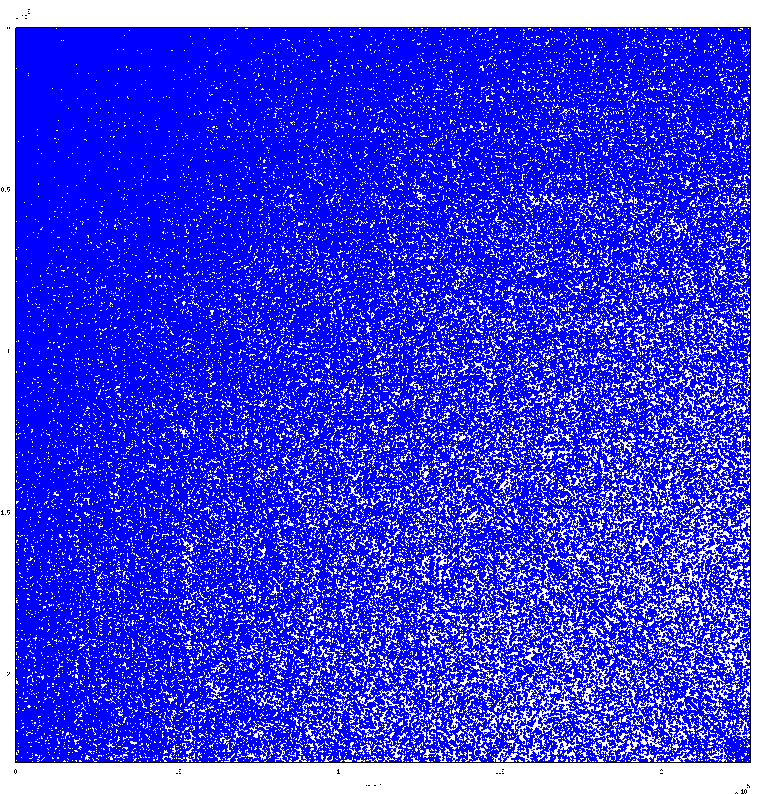
\includegraphics[scale=0.45]{img/coAuthorsCiteseer.pdf} }
%
%	\subfigure[\texttt{bcsstk30}]{ 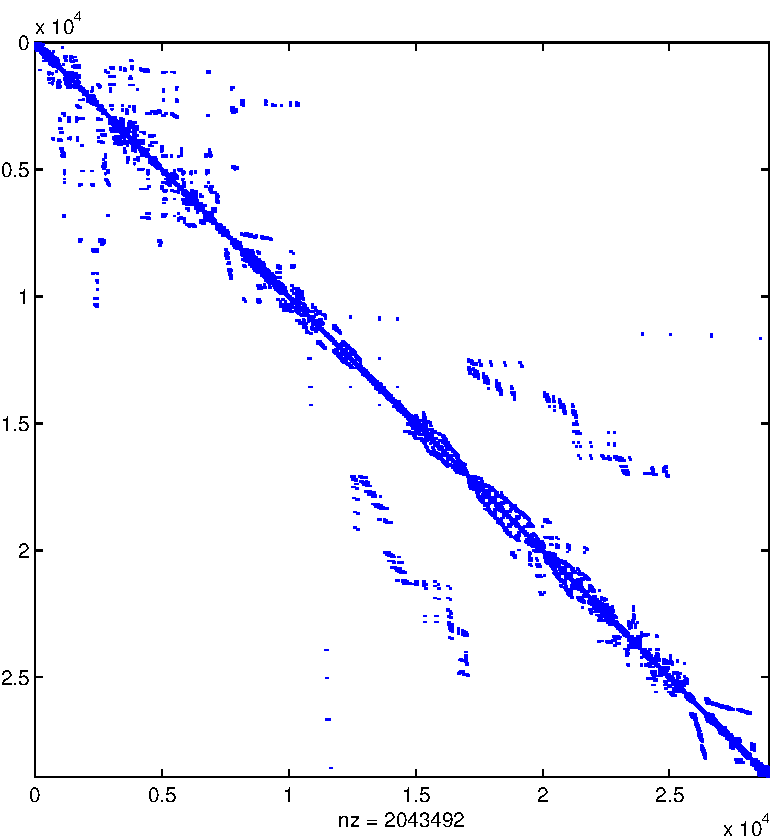
\includegraphics[scale=0.45]{img/bcsstk30.pdf} }
%	\subfigure[\texttt{bcsstk32}]{ 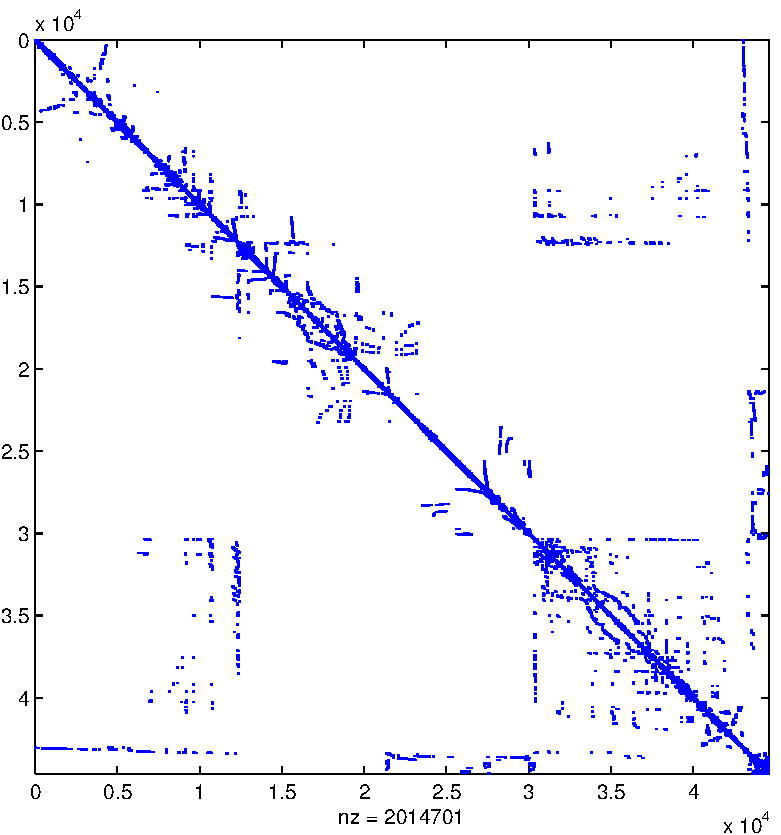
\includegraphics[scale=0.45]{img/bcsstk32.pdf} }
%	
%	\subfigure[\texttt{wave}]{ 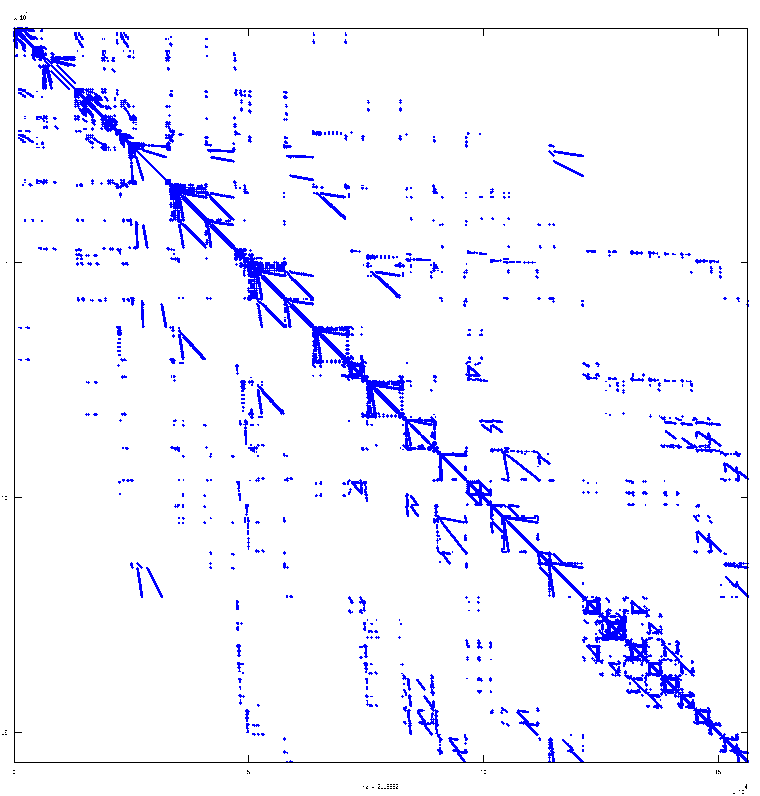
\includegraphics[scale=0.45]{img/wave.pdf} }
%	\subfigure[\texttt{tbdlinux}]{ 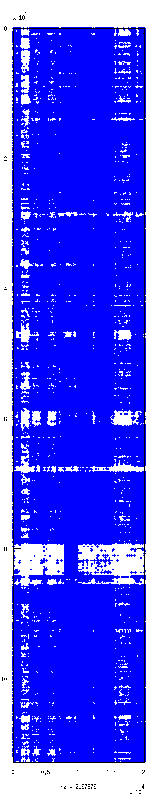
\includegraphics[scale=0.45]{img/tbdlinux.pdf} }
%	\caption{Sparsity patterns of the test matrices.} \label{fig:patterns2}
%\end{figure}
%
%\begin{figure}[h]
%	\centering
%	\subfigure[\texttt{rgg\_n\_2\_18\_s0}]{ 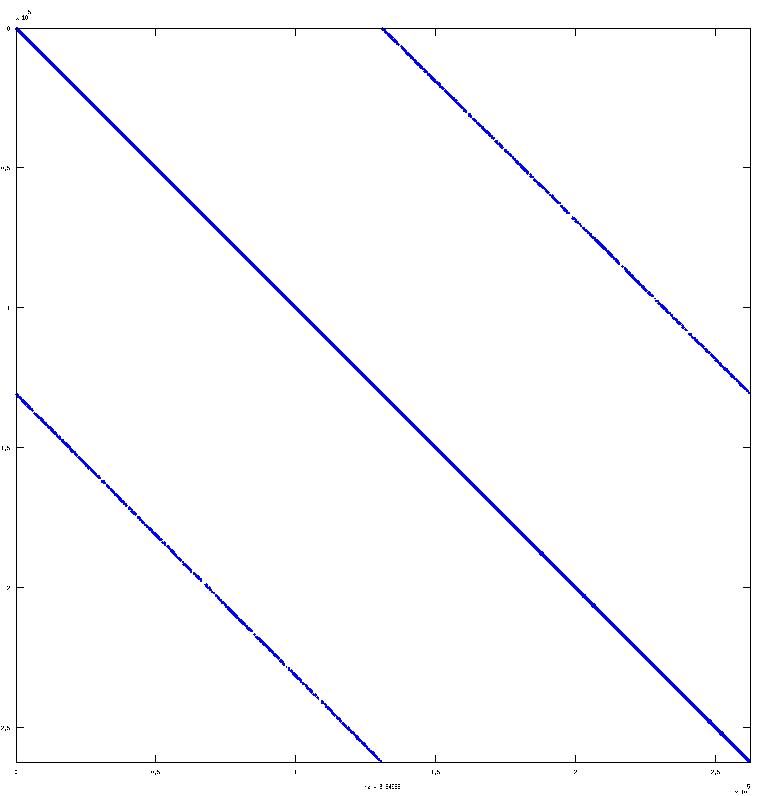
\includegraphics[scale=0.45]{img/rgg_n_2_18_s0.pdf} }
%	\subfigure[\texttt{belgium\_osm}]{ 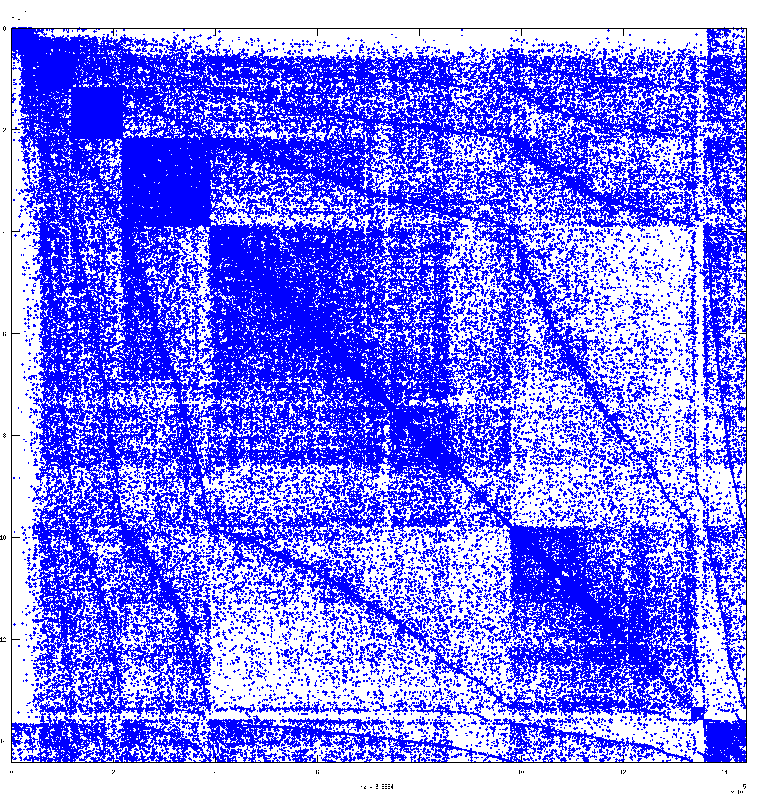
\includegraphics[scale=0.45]{img/belgium_osm.pdf} }
%	
%	\subfigure[\texttt{polyDFT}]{ 
\includegraphics[scale=0.45]{img/polyDFT.pdf} }
%	\subfigure[\texttt{netherlands\_osm}]{ 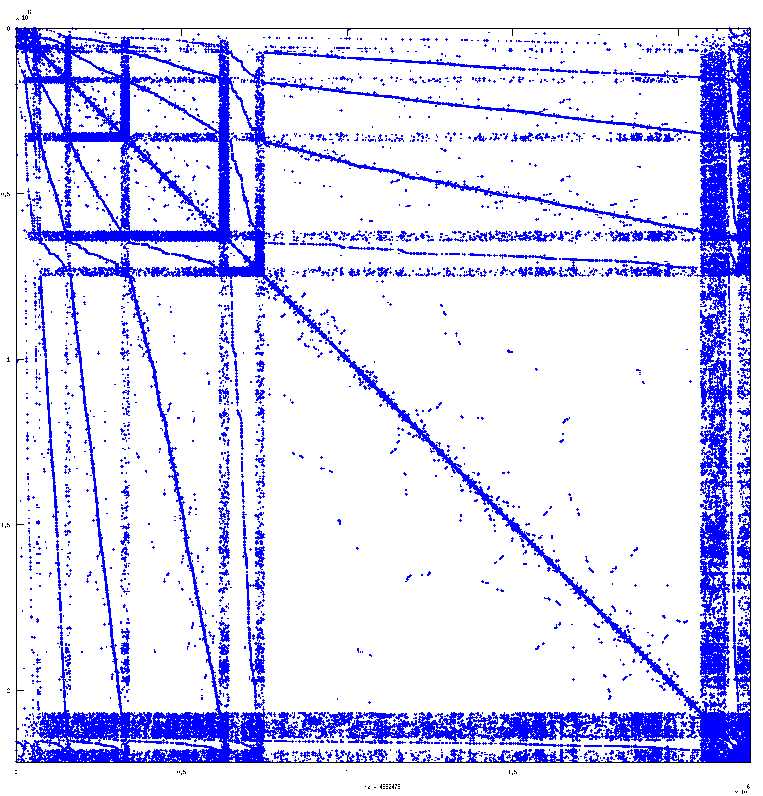
\includegraphics[scale=0.45]{img/netherlands_osm.pdf} }
%	
%	\subfigure[\texttt{cage13}]{ 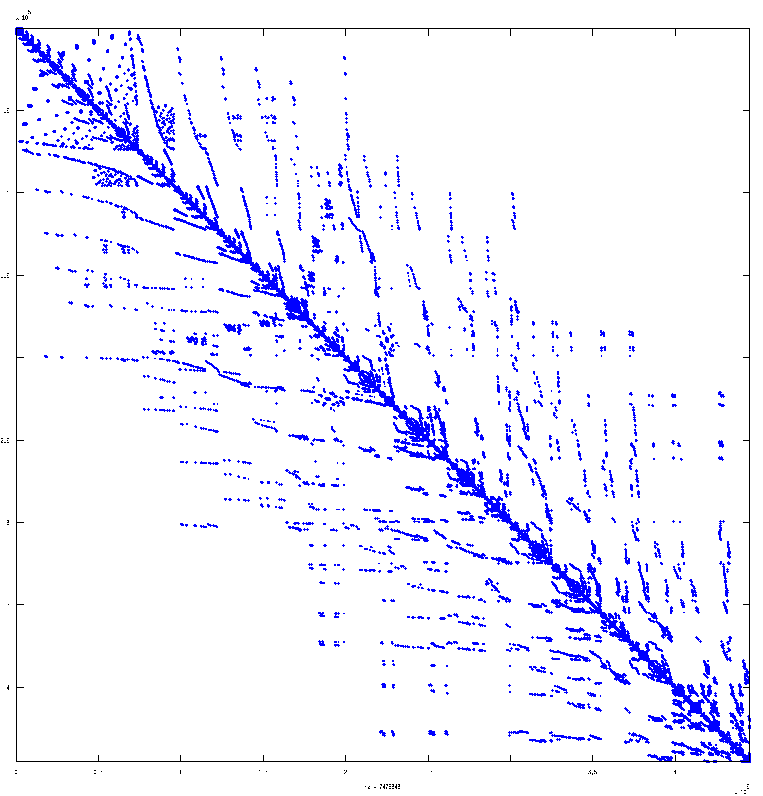
\includegraphics[scale=0.45]{img/cage13.pdf} }
%	\subfigure[\texttt{italy\_osm}]{ 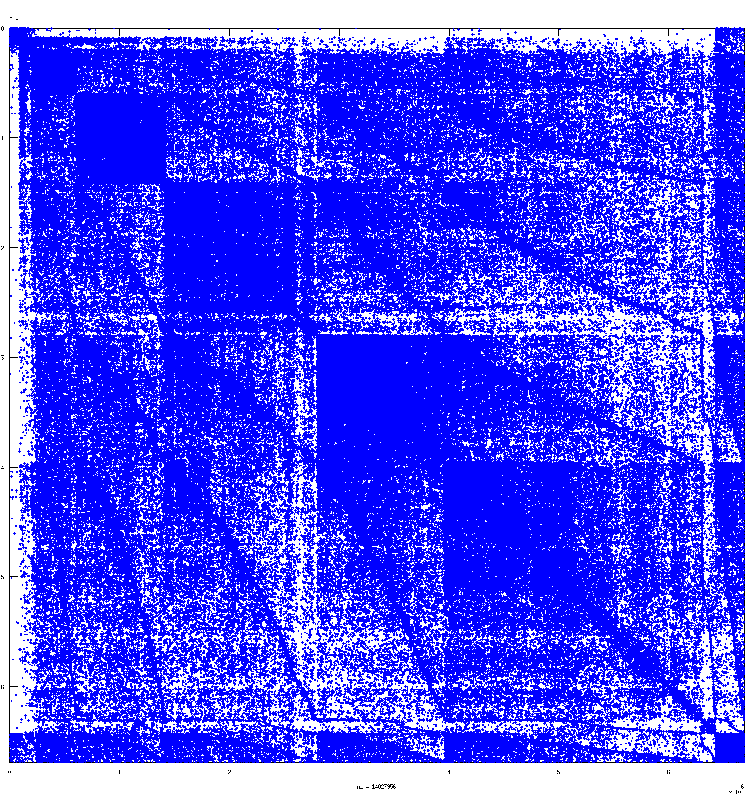
\includegraphics[scale=0.45]{img/italy_osm.pdf} }
%	\caption{Sparsity patterns of the test matrices.} \label{fig:patterns3}
%\end{figure}

\section{Preliminary selection of the best heuristics} \label{sec:preliminary_tests}

In Chapter \ref{chap:methods} and \ref{chap:independent_set} we discussed many heuristics, which in turn depend on different parameters. It is best to perform a preliminary analysis to quickly figure out which produce the best solutions and should therefore be tested extensively, and the ones that should not be further considered.

For this reason, a small number of different matrices (with a relatively small number of nonzeros) has been selected from our choice of Table \ref{tab:matrices}: in particular the considered matrices, which have a different structure, are \verb|dfl001|, \verb|tbdlinux|, \verb|nug30|, \verb|rgg_n_2_18_s0|, \verb|bcsstk30|.

The local search heuristic given in Section \ref{sec:globalview}, quickly turned out to be far from effective, and therefore we decided to discard it altogether in the numerical experiments.

In the following tests, the parameter $iter_{max}$ has been set to 1, which means that we are only perfoming one iteration of our heuristic. The reason for this choice will become clear in Section \ref{sec:iter_max}; for now, we will just take advantage of the fact that performing only one iteration is relatively fast and we can quickly get an idea about the best heuristics.

\subsection{Partition-oblivious heuristics} \label{sec:preliminary_po}

Table \ref{tab:preliminary_po} summarizes the results of this preliminary analysis of the partition-oblivious heuristics for the 5 chosen matrices. In the first line, the results of the medium-grain with the algorithm proposed in \cite{mediumgrain} are given. The value $\rho$ represents the geometric mean of the results for a given heuristic, averaged over all matrices and normalized w.r.t. the default medium-grain method.

\begin{table}[h]
	\centering

	\renewcommand{\arraystretch}{1.2}
	\begin{tabular}{|l||c|c|c|c|c||c|}
		\hline
		\multirow{2}{*}{\textbf{Heuristic}} &  \multicolumn{5}{c||}{\textbf{Matrix}} & \multirow{2}{*}{$\rho$} \\ \cline{2-6}
		& \texttt{dfl001} & \texttt{nug30} & \texttt{bcsstk30} & \texttt{tbdlinux} & \texttt{rgg\_n\_2\_18\_s0} & \\ \hline
		medium-grain & 590 & 36262 & 552 & 8135 & 910 & 1.0 \\ \hline %2445
		\verb|po_localview|& \textbf{571} & 36665 & \textbf{598} & 8327 & 1160  & 1.07 \\  %2609.2
		\verb|po_unsorted_concat_row|& 1492 & 189689 & 653 & 15081 & 1098 & 2.04 \\ % 0 0 0 %4979.1
		\verb|po_unsorted_concat_col|& 589 & 38491  & 600 & 24024 & \textbf{1066} & 1.32 \\ % 0 1 0 %3224.1
		\verb|po_unsorted_random|& 1314 & 113070 & 1127 & 20154 & 1093 & 2.11 \\  % 2 0 0 %5169
		\verb|po_unsorted_mix_alt|& 1461 & 181216 & 715 & 27942 & 1104 & 2.32 \\  % 4 0 0 % 5666
		\verb|po_unsorted_mix_spr|& 1322 & 81915 & 759 & 18584 & 1122 & 1.81 \\  % 4 1 0 % 4434
		\verb|po_sorted_w_simple|& 597 & 38383 & 785  & 8307 & 1093 & 1.13 \\ % 6 0 0 % 2771
		\verb|po_sorted_nw_simple|& 606 & 38674 & 789 & \textbf{8301} & 1096 & 1.14 \\ % 6 1 0 % 2787
		\verb|po_sorted_w_concat_row|& 1486 & 189681 & 642 & 15082 & 1078 & 2.01 \\ % 8 1 0 % 4907
		\verb|po_sorted_w_concat_col|& 597 & 38655 & 621 & 24045 & 1068 & 1.33 \\  % 8 1 1 % 3261
		\verb|po_sorted_nw_concat_row|& 1496 & 189683 & 614 & 15086 & 1090 & 2.01 \\ % 8 0 0 % 4913
		\verb|po_sorted_nw_concat_col|& 593 & 38513 & 621 & 24005 & 1076 & 1.33 \\ % 8 0 1 % 3256
		\verb|po_sorted_w_mix_alt|& 1317 & 162549 & 790 & 23683 & 1091 & 2.19 \\ % 10 0 1 % 5346
		\verb|po_sorted_w_mix_spr|& 641 & 163013 & 782 & 23441 & 1093 & 1.88 \\ % 10 0 0 % 4615
		\verb|po_sorted_nw_mix_alt|& 1457 & 62273 & 797 & 15015 & 1096 & 1.69 \\ % 10 1 0  % 4122
		\verb|po_sorted_nw_mix_spr|& 719 & 62402 & 793 & 15072 & 1106 & 1.47 \\  % 10 1 1 % 3586
		\verb|po_is|& 594 & \textbf{30655} & 615 & 13286 & -  & 1.12 \\ % 3491 
		\hline
	\end{tabular}
	\caption{Results of the devised partition-oblivious heuristics for the five chosen matrices. In each column, we use boldface to highlight the best found partitioning (not considering the medium-grain value).} \label{tab:preliminary_po}
\end{table}

In the table there is no result for the heuristic \verb|po_is| and the  matrix \verb|rgg_n_2_18_s0|, because the maximum number of levels of recursion was reached before the algorithm completed.


The first method shown in the table, discussed in Section \ref{sec:localview}, shows the best results among these partition-oblivious heuristics. This is not surprising, as such algorithm is quite similar to the one originally proposed in \cite{mediumgrain}; \verb|po_localview| performs slightly worse (7\%, on average) than \verb|medium-grain| because the latter also includes an iterative refinement procedure \cite[Section 3.3]{mediumgrain}: after the partitioning is performed, the matrix $B$ is constructed by assigning all the nonzeros that belong to processor 0 to $A_r$ and the ones that belong to processor 1 to $A_c$, then the corresponding hypergraph is created and a single run of the Kernighan-Lin heuristic is performed; this procedure (which does not increase the communication value) is repeated until there are no more improvements, then the roles of $A_r$ and $A_c$ are inverted and the procedure is restarted. This fairly cheap scheme, computationally speaking, is repeated several times, until no further reduction can be obtained. 

From the table, it appears that the framework discussed in Section \ref{sec:hot_restart} is not particularly effective in this case: some methods result even in twice the communication volume, on average; the \verb|po_sorted_w_simple| and \verb|po_sorted_nw_simple| heuristics produce the best results with a communication volume, respectively, 13\% and 14\% worse than the reference value. Moreover, it appears that mixing rows and columns in the priority vector is not advisable: for the matrices \verb|dfl001| and \verb|ug_30|, for example, we obtain a communication volume 3-5 times higher than \verb|medium-grain|. 

The heuristic that employs the computation of the maximum independent set on the full matrix produces interesting results, especially with the matrix \verb|nug30|: the communication volume is, on average, 16\% lower than the one obtained with the medium-grain method; with the other matrices (in particular \verb|tbdlinux|), however, the results are not as satisfactory.

From this preliminary testing, we should choose the heuristic \verb|po_localview| and \verb|po_is| for further testing in Section \ref{sec:final_tests}

\subsection{Partition-aware heuristics} \label{sec:preliminary_pa}

In Table \ref{tab:preliminary_pa}, we summarize the results for the partition-aware heuristics. As now we are considering a fully iterative framework, it is best to explicitly give the average of the 20 initial partitionings (iteration 0) alongside the average of the 20 final results (iteration 1). The value $\rho$ represents, similarly as before, the geometric mean of the final results, normalized w.r.t. the average of the initial partitionings. 

\begin{table}[h]
	\centering
	\renewcommand{\arraystretch}{1.15}
	\begin{tabular}{|l|c||c|c|c|c|c||c|}
		\hline
		\multirow{2}{*}{\textbf{Heuristic}} & \multirow{2}{*}{$i$} &  \multicolumn{5}{|c||}{\textbf{Matrix}} & \multirow{2}{*}{$\rho$} \\ \cline{3-7}
		& & \texttt{dfl001} & \texttt{nug30} & \texttt{bcsstk30} & \texttt{tbdlinux} & \texttt{rgg\_n\_2\_18\_s0} & \\ \hline
		\verb|pa_localview| & 0 & 582 & 36224 & 537 & 8051 & 914 &   \\ % 2422
		& 1 & \textbf{575} & 36896 & 577 & 9934 & 2189 & 1.26 \\ \hline %3055

		\verb|pa_sbdview| & 0 & 590 & 36057 & 546 & 8112 & 899 & \\ % 2430
		& 1 & 1493 & 187241 & 699 & 19852 & 1074 & 2.17 \\ \hline % 5296

		\verb|pa_sbd2view| & 0 & 583 &  36123 & 542 & 8018 & 906 &  \\ % 2419
		& 1 & 1276 & 125009 & 1150 & 20757 & 1055 & 2.17 \\ \hline % 5258
		
		\verb|pa_unsorted_concat_row| & 0 & 584 & 36512 & 597 & 7934 & 929 & \\ % 1 0 * % 2480
		& 1 & 628 & 42581 & 641 & 7337 & 1088 & 1.07 \\\hline %2675 
		
		\verb|pa_unsorted_concat_col| & 0 & 589 & 35945 & 574 & 7999 & 898 & \\ % 1 1 * % 2445
		& 1 & 589 & 38862 & 602 & 10087 & 1069 & 1.11 \\\hline % 2718 
		
		\verb|pa_unsorted_random| & 0 & 591 & 36390 & 550 & 8044 & 909 & \\ % 3 * * % 2440
		& 1 & 622 & 36952 & 589 & 8383 & 1094 & 1.08 \\ \hline % 2623
		
		\verb|pa_unsorted_mix_alt| & 0 & 592 & 36097 & 536 & 8019 & 896 & \\ % 5 0 * % 2415
		& 1 &  633 & 40286 & 684 & 9683 & 1108 & 1.18 \\ \hline % 2847
		
		\verb|pa_unsorted_mix_spr| & 0 & 589 & 36137 & 542 & 8024 & 905 & \\ % 5 1 * % 2415
		& 1 &  642 & 39703 & 645 & 8361 & 1094 & 1.13 \\ \hline % 2726
		
		\verb|pa_sorted_w_simple| & 0 & 587 & 36498 & 566 & 8018 & 903 & \\ % 7 1 * % 2446 
		& 1 &  586 & 38730 & 577 & 7992 & 1102 & 1.06 \\ \hline % 2585
		
		\verb|pa_sorted_nw_simple| & 0 & 596 & 35837 & 568 & 8014 & 882 & \\ % 7 0 * % 2435
		& 1 &  594 & 38683 & 578 & 8004 & 1100 & 1.06 \\ \hline % 2592
		
		\verb|pa_sorted_w_concat_row| & 0 & 585 & 36158 & 556 & 8019 & 880 & \\ % 9 1 0 % 2420
		& 1 &  621 & 44930 & 617 & 7349 & 1071& 1.10 \\ \hline % 2669
		
		\verb|pa_sorted_w_concat_col| & 0 & 595 & 36157 & 545 & 7995 & 908 &  \\ % 9 1 1 % 2432
		& 1 &  596 & 38823 & 633 & 10108 & 1075 & 1.13 \\ \hline % 2757
		
		\verb|pa_sorted_nw_concat_row| & 0 & 598 & 36661 & 548 & 8025 & 889 & \\ % 9 0 0 % 2436
		& 1 & 638 & 42580 & 601 & 7359 & 1066 & 1.08 \\ \hline % 2639
		
		\verb|pa_sorted_nw_concat_col| & 0 & 580 & 36421 & 561 & 8035 & 916 & \\ % 9 0 1 % 2444
		& 1 & 595 & 38614 & 617 &  10084  & 1077 & 1.12 \\ \hline % 2738
		
		\verb|pa_sorted_w_mix_alt| & 0 &  586 & 36566 & 549 & 8006  & 912 & \\ % 11 0 1 % 2436
		& 1 & 692 & 41963 & 593 & 9476 & 1105 & 1.16 \\ \hline % 2826
		
		\verb|pa_sorted_w_mix_spr| & 0 &  593 & 36085 &  537 & 8010 & 924 & \\ % 11 1 1 % 2431
		& 1 & 619 & 39697 & 571 &  9060 & 1078 & 1.10 \\ \hline % 2675
		
		\verb|pa_sorted_nw_mix_alt| & 0 & 588 & 36509 & 546 & 8020 & 891 & \\ % 11 0 0 % 2424
		& 1 &  687 & 42542 & \textbf{566} & 9486 & 1085 & 1.15 \\ \hline % 2794
		
		\verb|pa_sorted_nw_mix_spr| & 0 & 589 & 36197 & 553 & 8006  & 886 & \\ % 11 1 0 % 2424
		& 1 &  655 & 39201 & 602 & 9076 & 1094 & 1.13 \\ \hline % 2737
		
		\verb|pa_is_1| & 0 & 592 & 36716 & 534 & 7997 & & \\ % 3104
		& 1 & 588 & \textbf{36118} & 614 & \textbf{7323} & - & 1.01 \\ \hline % 3126
		
		\verb|pa_is_2| & 0 & 596 & 35972 &  539 & 8011 &  & \\ % 3101
		& 1 & 592 & 36375 &  631 & 8681 & - & 1.06 \\ \hline % 3296
		
		\verb|pa_is_3| & 0 & 590 & 36432 & 540 & 7997 & & \\ % 3104
		& 1 & 589 & 36324 & 635 & 7410 & - & 1.02\\ \hline % 3168

	\end{tabular}
	\caption{Results for partition-oblivious heuristics. Boldface is used to highlight the best found partitioning for each matrix. Iteration 0 corresponds to the average of the initial partitionings, whereas iteration 1 is the average of the final partitionings. In the last column, for each method, the geometric mean of iteration 1 is normalized w.r.t. the geometric mean of iteration 0.} \label{tab:preliminary_pa}
\end{table}

The computation of the independent set was, once again, not possible with \verb|rgg_n_2_18_s0|, because the maximum level of recursion was reached before being able to finish the algorithm.

From the table, it appears that the approaches discussed in Section \ref{sec:sbd} are not effective: in both cases (using the SBD and SBD2 forms of the partitioned matrix) the communication volume is, on average, more than twice the one obtained with the medium-grain method. 

Regarding the framework discussed in Section \ref{sec:hot_restart}, differently from the partition-oblivious case, it seems that mixing rows and columns does not produce a sharp decrease in the quality of the solutions, albeit being far from being a good result: if no sorting is performed, the communication volume is on average 18\% and 13\% higher (depending on the mixing strategy), whereas with sorting we have a 10\% and 16\% worse solution.

Moreover, it appears that moving the indices with one nonzero at the back of our priority vector (denoted by \verb|w| in the heuristics) or not (denoted by \verb|nw|) does not yield a substantial difference; in addition, there is no clear advantage of one strategy over the other, and therefore, should we decide to consider these methods for further testing, only one of the two strategies should be picked.

The good results produced by the heuristics \verb|pa_unsorted_concat_row| and \verb|pa_unsorted_concat_col| (and their sorted counterparts, which do not produce a significantly different result) are a bit surprising: we expected that a more elaborate strategy (for example, sorting and mixing of rows and columns) would yield a lower communication volume than the simple concatenation of rows and columns. These two methods, especially for strongly rectangular matrices, produce fairly low communication volumes, if we start the concatenation with the longer dimension. If there are more rows than columns, for example, it means that the rows are in general shorter, and therefore, by giving them high priority, we have a higher chance that keeping all of their nonzero together will not cause communication also for the columns. From another point of view, we could interpret this heuristic in the light of Chapter \ref{chap:independent_set}: the set of indices of the rows (or the columns) is in fact an independent set, as it is obvious that two rows (or columns) do not share any nonzero; this means that, in these two heuristics, we are roughly doing the same as in Section \ref{sec:is_vector}, albeit not as targeted to cut and uncut indices. 

The behavior of these two heuristics is also consistent with the size of the matrix: if one produces good results, the other performs much worse. This suggest us that these two schemes could be merged in a single method, \verb|pa_localbest|, which internally decides which one of the two is to be used, based on the number of rows and columns of the matrix. This is very similar to the \verb|localbest| method (hence the name) employed by Mondriaan, in which the size of the matrix determines whether the row-net or the colum-net method is applied.

The computation of the maximum independent set on the uncut indices seems to be an effective strategy for a fully iterative partitioning scheme, especially the heuristic \verb|po_is_1|. The average of the partitionings is indeed very close to the one obtained with the medium-grain model (rounded up, only 1\% higher) and we have a definite improvement for the matrix \verb|tbdlinux|, where the communication volume is 8\% lower.

In general, we can see how with these partition-aware heuristics the results are better than with the partition-oblivious ones: the value of $\rho$ is, in general, closer to 1. This means that, in order to select the best of partition-aware methods, we need to be stricter: \verb|pa_unsorted_concat_row| and \verb|pa_unsorted_concat_col| (for which we will drop the label \verb|unsorted_concat|, as \verb|row| or \verb|col| is sufficient to distinguish from the others), the \verb|pa_localbest| scheme defined as above, \verb|pa_sorted_w_simple| (which we will denote simply by \verb|pa_simple|), \verb|pa_is_1| and \verb|pa_is_3| are selected for further testing in Section \ref{sec:final_tests}.

\section{Number of iterations} \label{sec:iter_max}

The parameter $iter_{max}$ of Algorithm \ref{alg:framework} is of vital importance for the running time of our iterative method: our research motivation, for the partition-aware heuristics, is to trade computation time for solution quality, but efficiency is also a fundamental goal. An iterative scheme in which each iteration is only a slight improvement on the previous one (which means that the heuristic needs a high value of $iter_{max}$ to attain a low communication value), is less desirable than a scheme that attains a similarly low communication value in just one or two iterations. Note that this reasoning only applies to partition-aware heuristics, as the partition-oblivious ones are not fully iterative: $iter_{max}$, in this case, means that a number of independent iterations is performed.

Luckily enough, the heuristics introduced in Chapters \ref{chap:methods} and \ref{chap:independent_set} fall, more or less, in this last category: whenever a good improvement over initial partitioning can be achieved, it usually happens in the first iteration; the solution quality, over the next few ones, either remains more or less constant, or gets worse. This is the main reason why in Section \ref{sec:preliminary_tests}, for the partition-aware heuristics, we set the parameter $iter_{max}$ to 1, other than conveniently saving computation time.

In Table \ref{tab:iterations}, we show the results of multiple iterations for some of the selected heuristic of Section \ref{sec:preliminary_pa}. We replaced the matrix \verb|rgg_n_2_18_s0| with the matrix \verb|delaunay_n15| because, as seen previously, the heuristics which computed the maximum independent set failed to return a solution.

We use a simplified notation for the heuristics in this table: \verb|pa_row| and \verb|pa_col| instead, respectively, of \verb|pa_unsorted_concat_row| and \verb|pa_unsorted_concat_col|, and, likewise, we use \verb|pa_simple| instead of \verb|pa_sorted_w_simple|.

\begin{sidewaystable}[h]
	\centering
	\renewcommand{\arraystretch}{1.2}
	\begin{tabular}{|c|l|c||c|c|c|c|c|c|c|c|c|c|}
		\hline
		\multirow{2}{*}{\textbf{Matrix}} &\multirow{2}{*}{\textbf{Heuristic}} & \multicolumn{11}{c|}{\textbf{Iterations}} \\ \cline{3-13} 
		&& 0 & 1 & 2 & 3 & 4 & 5 & 6 & 7 & 8 & 9 & 10 \\ \hline
		\multirow{5}{*}{\texttt{dfl001}}		&\verb|pa_row| & 598 & 631 & 696 & 759 & 806 & 798 & 837 & 818 & 855 & 881 & 874 \\ 
		&\verb|pa_col| &  587&  590 & 594 & 586 & 596 & 593 & 595 & 594 & 594 & 602 & 596 \\ 
		&\verb|pa_simple| & 589 & 602 & 601 & 597 & 587 & 602 & 593 & 591 & 602 & 600 & 594 \\
		&\verb|pa_is_1| & 599 & 593 & 586 & 597 & 592 & 598 & 607 & 592 & 587 & 587  & 601 \\
		&\verb|pa_is_3| & 597 & 600 & 594 & 589 & 600 & 601 & 592 & 594 & 594 & 593 & 590 \\
		\hline
		\multirow{5}{*}{\texttt{nug30}}		&\verb|pa_row| & 	36308 & 41522 & 58016 & 57194 & 60054 & 60361 & 62408 & 63244 & 63699 & 64994 & 66534 \\ 
		&\verb|pa_col| & 36059 & 32965&  31550 & 31335 & 31390 & 31009 & 30881 & 30709 & 30437 & 30924 & 31345 \\
		&\verb|pa_simple| & 37158 & 37051 & 37515 & 37723 & 37389 & 37732 & 37683 & 37660 & 37613 & 37491 & 37681 \\
		&\verb|pa_is_1| & 	36649 & 36828 & 36849 & 36976 & 36856 & 36894 & 36970 & 37105 & 36851 & 36989 & 36440 \\
		&\verb|pa_is_3| & 35793 & 36191 & 35975 & 36190 & 36054 & 36219 & 36235 & 36432 & 36159 & 35671 & 36020 \\ \hline
		\multirow{5}{*}{\texttt{bcsstk30}}		&\verb|pa_row| &  562 & 670 & 581&  638 &  599 &  604 &  674 &  727&   584&   673 &  607 \\ 
		&\verb|pa_col| & 540 &  620 & 624 & 603 & 676 & 662 & 682 & 685 & 586 & 630 & 595 \\ 
		&\verb|pa_simple| &544 & 677 & 554 & 543 & 543 & 546 & 541 & 541 & 534 & 544 & 528 \\
		&\verb|pa_is_1| & 562 & 574 & 563 & 614 & 570 & 567 & 593 & 693 & 612 & 646 & 595 \\
		&\verb|pa_is_3| &542 & 658 & 626 & 727 & 597 & 646 & 672 & 618 & 669 & 616 & 626 \\ \hline
		\multirow{5}{*}{\texttt{tbdlinux}}		&\verb|pa_row| & 8023 & 7365  & 7996  & 7977  & 8402  & 9527 & 10127 & 11141 & 11846 & 12059 & 12327 \\ 
		&\verb|pa_col| & 8108 & 10040  & 9447  & 9614  & 9732  & 9872  & 9955 & 10079 & 10171 & 10268 & 10327 \\ 
		&\verb|pa_simple| & 8044 & 8027 & 8002 & 7964 & 7958 & 7964 & 7957 & 7951 & 7934 & 7979 & 7956 \\
		&\verb|pa_is_1| & 8055 & 7343 & 7361 & 7360 & 7343 & 7375 & 7330 & 7365 & 7357 & 7331 & 7358 \\
		&\verb|pa_is_3| & 8069 & 7432 & 7426 & 7446 & 7445 & 7432 & 7444 & 7440 & 7461 & 7431 & 7443 \\ \hline
		\multirow{5}{*}{\texttt{delaunay\_n15}}		&\verb|pa_row| & 312 & 363 &  350 &  358 &  349 &  353 &  357 &  354  & 359 &  360 &  360 \\ 
		&\verb|pa_col| & 315 & 354 & 359 & 352 & 355 & 350 & 361 & 352 & 355 & 364 & 357 \\ 
		&\verb|pa_simple| & 313 & 340 & 333 & 339 & 329 & 330 & 326 & 335 & 337 & 331 & 339 \\
		&\verb|pa_is_1| & 308 & 362 & 374 & 371 & 364 & 362 & 369 & 364 & 364 & 360 & 369 \\
		&\verb|pa_is_3| & 305 & 357 & 363 & 364 & 369 & 362 & 379 & 375 & 361 & 374 & 369 \\\hline
		\end{tabular}
	\caption{Multiple iterations of the four selected partion-aware heuristics. The numbers shown are the rounded arithmetic means of each iteration over 10 repeats of the experiment. Iteration 0 stands for the initial partitioning obtained with the medium-grain model.} \label{tab:iterations}
\end{sidewaystable}

Figure \ref{fig:iterations} shows the contents of Table \ref{tab:iterations} in a graphical way: each communication volume has been normalized w.r.t. the initial partitioning, in order to better understand whether there is an improvement or not, over 10 iterations of the heuristic.

\begin{figure}[h]
	\centering
	\subfigure[\texttt{dfl001}]{ 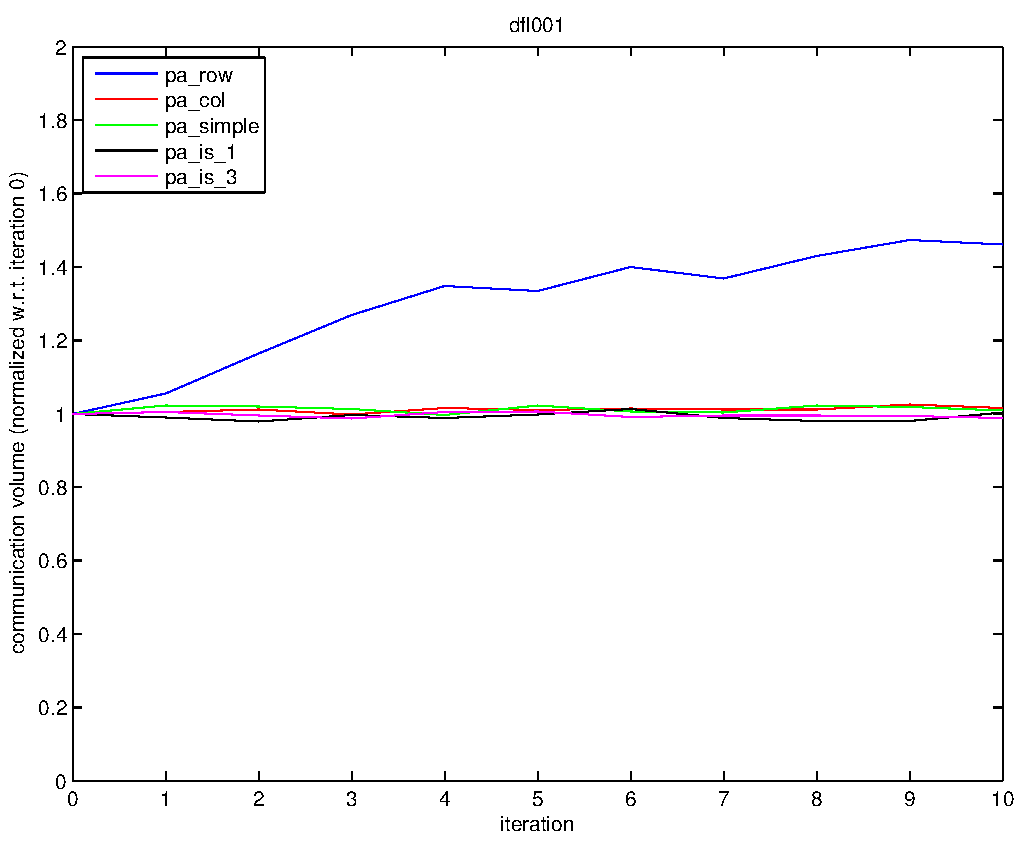
\includegraphics[scale=0.6]{img/iter_dfl.pdf} }
	\subfigure[\texttt{nug30}]{ 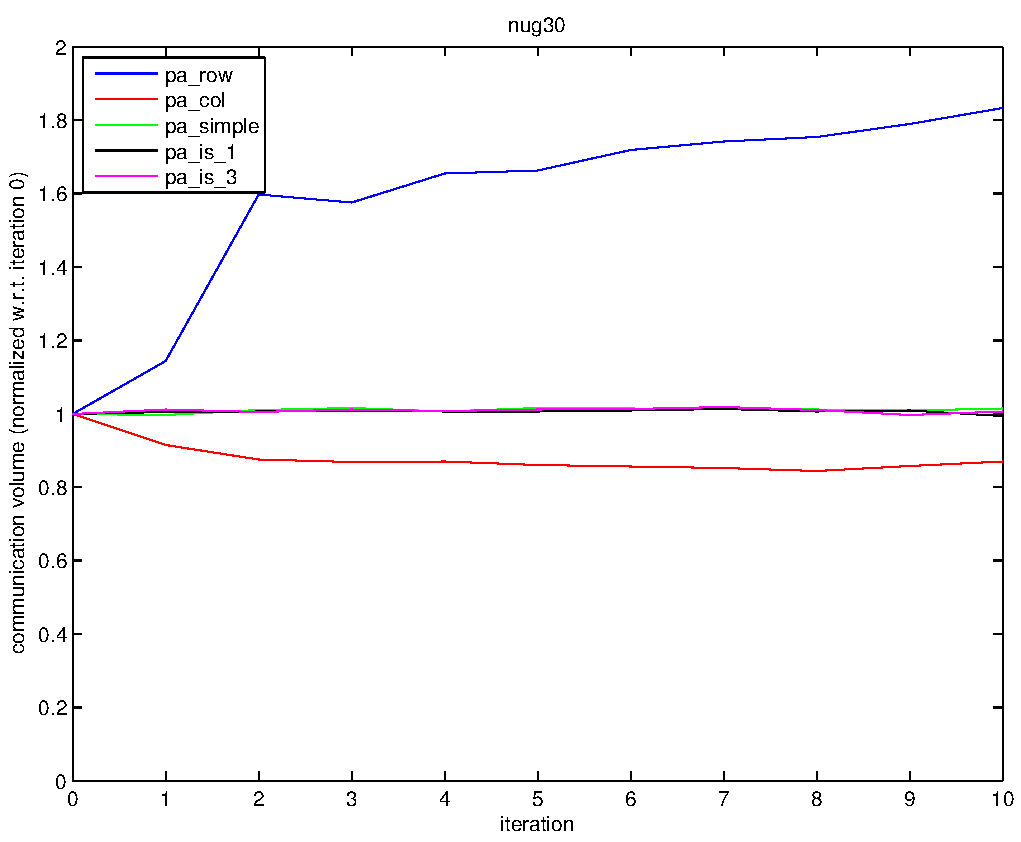
\includegraphics[scale=0.6]{img/iter_nug30.pdf} }
\end{figure}

\begin{figure}[h]
\centering
	\subfigure[\texttt{bcsstk30}]{ 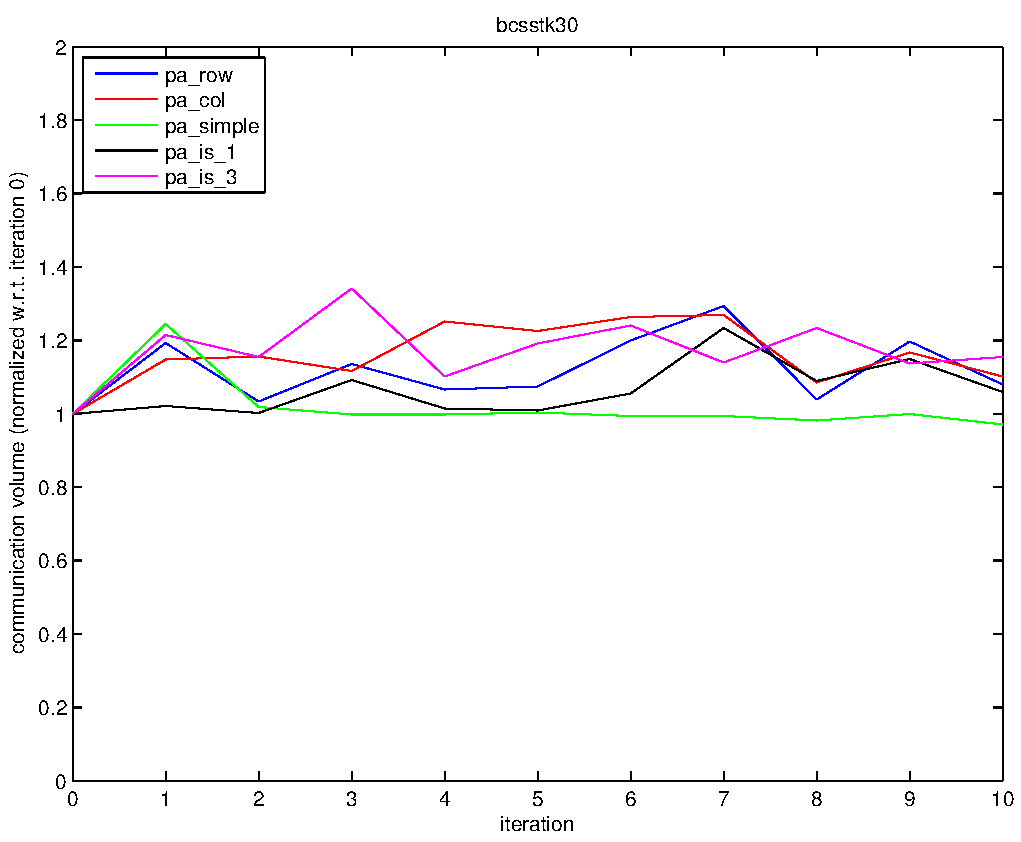
\includegraphics[scale=0.6]{img/iter_bcs.pdf} }
	\subfigure[\texttt{tbdlinux}]{ 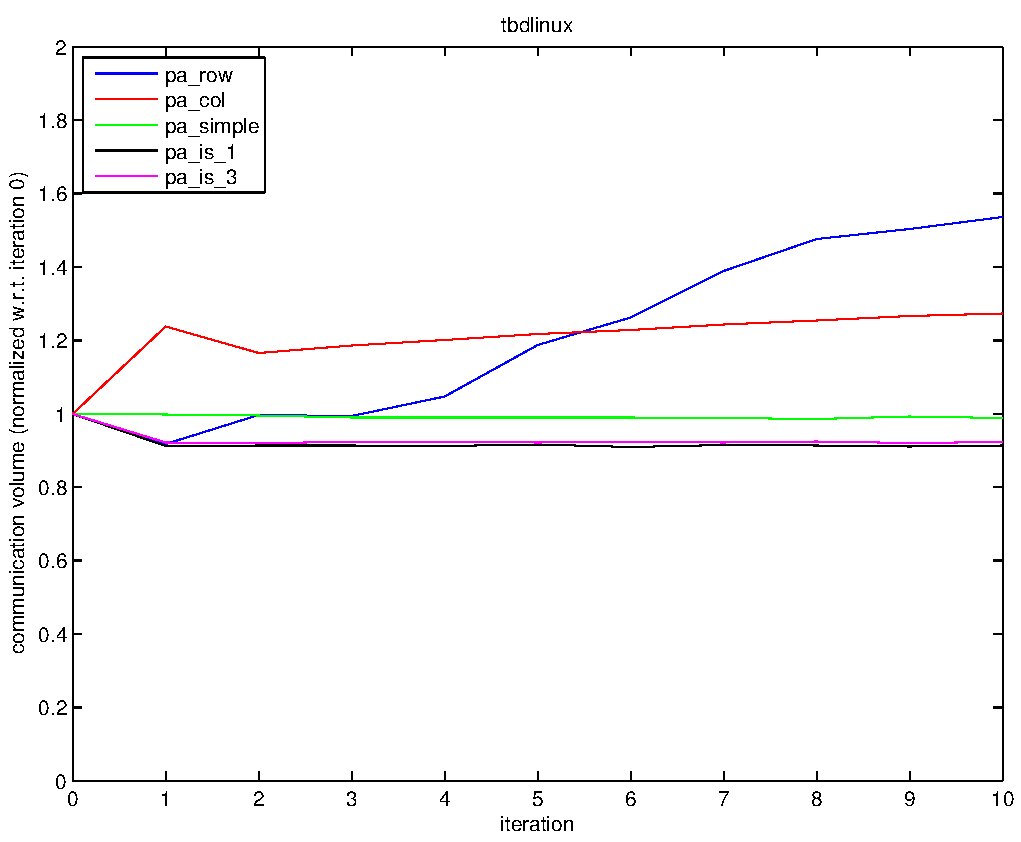
\includegraphics[scale=0.6]{img/iter_tbdlinux.pdf} }
\end{figure}

\begin{figure}[h]
	\centering
	\subfigure[\texttt{delaunay\_n15}]{ 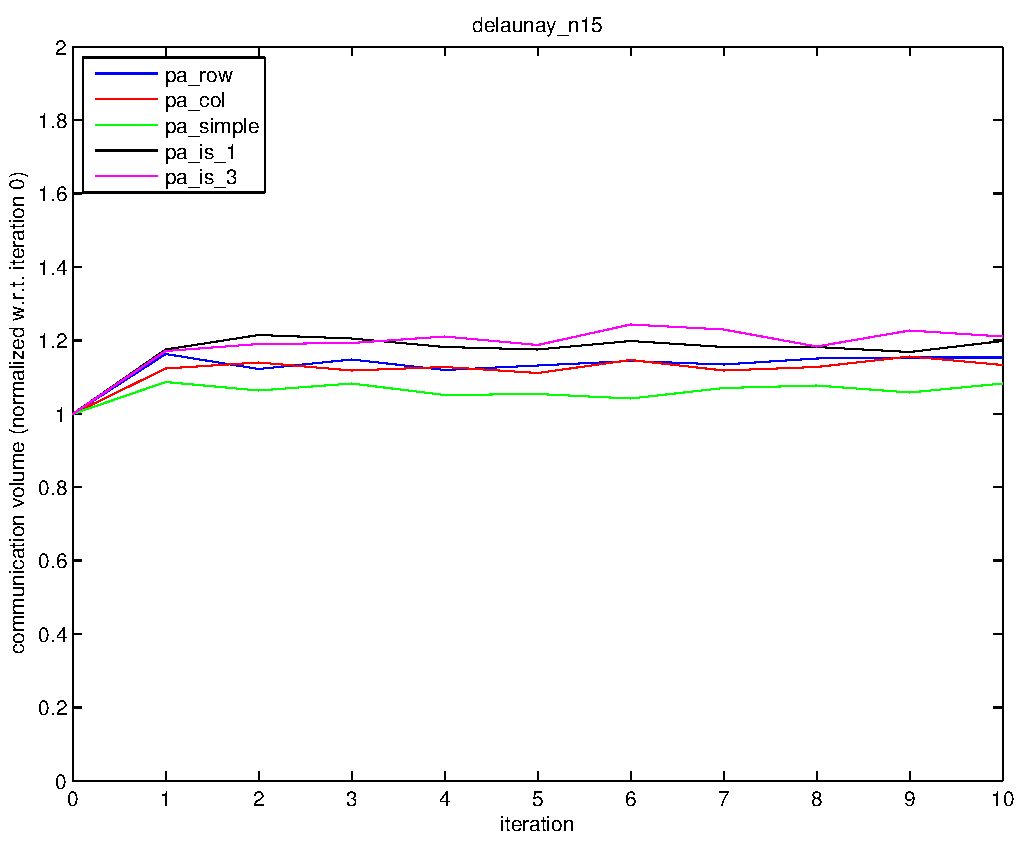
\includegraphics[scale=0.6]{img/iter_delaunay.pdf} }
	\caption{Graphical visualization of Table \ref{tab:iterations}. Each value has been normalized w.r.t. the first iteration. } \label{fig:iterations}
\end{figure}

It seems there is no clear advantage in performing 10 iterations over just one, except for the combination \verb|pa_unsorted_concat_col| and \verb|nug30|: but even in this case, after improving the first two iterations, the communication value somewhat stagnates around 30500-31000.

For some of pairs heuristic-matrix which produced good results in Section \ref{sec:preliminary_pa}, (namely \verb|pa_is_1| and \verb|pa_is_3| for the matrix \verb|tbdlinux|), we can see that the communication volume, after improving quickly in the first iteration from the initial partitioning, stays at the same levels. In most of the other cases, 10 iterations do not improve significantly the value attained at the first iteration, or they even make it significantly worse.

\section{Analysis of the performance of the best heuristics through the test matrices} \label{sec:final_tests}

In Section \ref{sec:preliminary_tests} we selected the most interesting heuristic for the final round of tests. In this section, we will check the quality of these methods for all of the matrices discussed in Section \ref{sec:test_matrices}.

The testing is performed exactly as before: 20 initial partitionings, and for each 5 runs of a single iteration of the considered heuristic. The means are computed as in Section \ref{sec:preliminary_tests}.

\subsection{Partition-oblivious heuristics}

The results for the partition-oblivious heuristics can be found in Table \ref{tab:final_po}.

\begin{table}[h]
	\renewcommand{\arraystretch}{1.3}
	\centering
	\begin{tabular}{|l|x{2.8cm}|x{2.8cm}|x{2.8cm}|}
	\hline
	\multirow{2}{*}{\textbf{Matrix}} & \multicolumn{3}{c|}{\textbf{Heuristic}} \\ \cline{2-4}
	& \texttt{medium-grain} &  \texttt{po\_localview} & \texttt{po\_is} \\\hline
	\verb|lpi_ceria3d| & \textbf{220} & 239 & 1030 \\
	\verb|dfl001| & 590 & \textbf{571} & 594  \\
	\verb|delaunay_n15| & \textbf{310} & 338 & 367 \\
	\verb|deltaX| & 236 & \textbf{222} & 586 \\
	\verb|cre_b| & \textbf{580} & 630 & 632 \\
	\verb|tbdmatlab| & \textbf{3951} & 4276 & 4711 \\
	\verb|nug30| & 36262 & 36665 & \textbf{30655} \\
	\verb|coAuthorsCiteseer| & \textbf{9583} & 10459 & 16217 \\
	\verb|bcsstk30| & \textbf{552} & 598 & 615 \\
	\verb|bcsstk32| &  \textbf{818} & 993 & 1082 \\
	\verb|wave| & \textbf{4624} & 5660 & 5100 \\
	\verb|tbdlinux| & \textbf{8135} & 8327 & 13286\\
	\verb|rgg_n_2_18_s0| & \textbf{910} & 1160 & - \\
	\verb|belgium_osm| & 248 & 264 & \textbf{263} \\
	\verb|polyDFT| & 3633 & 3701 & $\textbf{3456}^*$ \\
	\verb|netherlands_osm| & \textbf{194} & 204 & 215 \\
	\verb|cage13| & \textbf{45233} & 52109 & 57556 \\
	\verb|italy_osm| & \textbf{262} & 280 & 284 \\ \hline
	% 1371 & 1468 &&& 1488 & 1826
	\multicolumn{1}{|r|}{$\rho$}	& 1.0 & 1.07 & 1.22\\ \hline
\end{tabular}
\caption{Results of the selected partition-oblivious heuristics with the test matrices. For each matrix, the best found average partitioning is highlighted.} \label{tab:final_po}
\end{table}

First of all, we can see that the value of $\rho$ attained by the heuristic \verb|po_localview| is indeed very similar to the one obtained in Section \ref{sec:preliminary_tests}, which suggests us that the preliminary matrices were indeed a good sample of the whole test set, at least for this heuristic. Regarding \verb|po_is|, instead, we can see that now the final value of $\rho$ is much higher: this is to be explained from the fact that in the preliminary tests one of the matrices did not yield any result, and therefore the average was computed only on four matrices, and among those there was the matrix for which this heuristic performs best, \verb|nug30|, which therefore had a lot of weight. Now that there is a wide variety of matrices, the good result attained for \verb|nug30| has a lower weight, and the performance of this method with the other matrices are not particularly satisfactory.

It is interesting to note that this heuristic that employs the computation of the independent set has somewhat of an erratic behavior: in a few matrices (\verb|nug30|, \verb|polyDFT|) the communication value is the lowest among the three methods considered (respectively 16\% and 5\% lower than the second best method, \verb|medium-grain|), whereas on other matrices (\verb|lpi_ceria3d|, \verb|tbdlinux|, \verb|coAuthorsCiteseer|) the final solution is much worse.

It it interesting to highlight a particular result of the table: we marked with the symbol $*$ the solution attained by \verb|po_is| for the matrix \verb|polyDFT| because, for every initial partitioning with medium-grain, each independent iteration with the heuristic produced the same communication value of 3456, the lowest recorded. This suggest that either this value is a local optima in which it is particulary easy to get stuck with, or the optimal value.

\subsection{Partition-aware heuristics}

Table \ref{tab:final_pa} shows the final results for the partition-aware heuristics, with all the matrices from Section \ref{sec:test_matrices}. We used simplified labels for the considered heuristics, as there is no possible confusion among those. \verb|pa_row| and \verb|pa_col| represent, respectively, \verb|pa_unsorted_concat_row| and \verb|pa_unsorted_concat_col|, whereas \verb|pa_simple| represents \verb|pa_sorted_w_simple|.

\begin{sidewaystable}[h]
	\begin{tabular}{|l|c|c||c|c||c|c||c|c||c|c||c|c|}
	\hline
	\multirow{3}{*}{\textbf{Matrix}} & \multicolumn{12}{c|}{\textbf{Heuristic}} \\ \cline{2-13}
	& \multicolumn{2}{c||}{\texttt{pa\_row}} &  \multicolumn{2}{c||}{\texttt{pa\_col}} & \multicolumn{2}{c||}{\texttt{pa\_localbest}} & \multicolumn{2}{c||}{\texttt{pa\_simple}} & \multicolumn{2}{c||}{\texttt{pa\_is\_1}} & \multicolumn{2}{c|}{\texttt{pa\_is\_3}} \\\cline{2-13}
	& initial & final & initial & final & initial & final & initial & final & initial & final & initial & final \\ \hline
	\verb|lpi_ceria3d| & 225 & 225 & 223 & 243 & 223 & 225 &  224 & 229 & \textbf{221} & 229 & 222 & 222 \\
	\verb|dfl001| & \textbf{584} & 628 & 589 & 589 & 589 & 589 & 587 & 586 & 593 & 589 & 590 & 589 \\
	\verb|delaunay_n15| & 310 & 350 & \textbf{306} & 362 & 310 & 350 & 312 & 333 & 309 & 365 & 309 & 367\\
	\verb|deltaX| & 236 & 224 & 236 & 227 & 236 & 224 & 234 & \textbf{222} & 235 & 223 & 237 & 224 \\
	\verb|cre_b| & 602 & 1014 & 599 & 637 & 599 & 637 & \textbf{590} & 627 & 590 & 649 & 590 & 627 \\
	\verb|tbdmatlab|& 3884 & 3623 & 3934 & 4096 & 3884 & \textbf{3623} & 3878 & 3903 & 3928 & 3739 & 3939 & 3677 \\
	\verb|nug30| & 36512 & 42581 & 35945 & 38862 & \textbf{35945} & 38862 & 36498 & 38731 & 36716 & 36119 & 36432 & 36324 \\
	\verb|coAuthorsCiteseer| & 9534 & 9885 & 9697 & 10050 & 9534 & 9885 & 9633 & 9955 & \textbf{9523} & 10049 & 9528 & 14737 \\
	\verb|bcsstk30| & 597 & 641 & 574 & 602 & 574 & 602 & 567 & 577 & \textbf{535} & 614 & 540 & 636 \\
	\verb|bcsstk32| & 804 & 958 & 837 & 1022 & \textbf{804} & 958 & 818 & 944 & 903 & 1037 & 850 & 1003 \\
	\verb|wave| & 4737 & 4893 & 4782 & 4893 & 4782 & 4893 & 4725 & 5427 & 4689 & 5099 & \textbf{4650} & 5199 \\
	\verb|tbdlinux| &  7984 & 7337 & 7999 & 10086 & 7984 & 7337 & 8018 & 7992 & 7998 & \textbf{7323} & 7997 & 7410 \\
	\verb|rgg_n_2_18_s0| & 928 & 1088 & 897 & 1069 & \textbf{897} & 1069 & 903 & 1102 & - & - & - & - \\
	\verb|belgium_osm| & 227 & 258 & 255 & 266 & \textbf{227} & 258 &  282 & 251 & 247 & 248 & 242 & 260 \\
	\verb|polyDFT| & 3643 & 3616 & 3732 & 3607 & 3732 &  3607 & 3725 & 3729 & 3648 & \textbf{3508} & 3629 & 3515 \\
	\verb|netherlands_osm| & 204 & 190 & \textbf{175} & 191 & 204 & 190 & 191 & 199 & 194 & 199 & 192 & 210 \\
	\verb|cage13| & 45845 & 54155 & 45405 & 52251 & 45405 & 52251 & 45686 & 49784 & \textbf{45252} & 57117 & 45314 & 57181\\
	\verb|italy_osm| & 254 & 278 & 262 & 278 &262 & 278 & 279 & 284 & 267 & 277 & &  \\ \hline
	\multicolumn{1}{|r|}{$\rho$}	& 1.0  & 1.08 & 1.0  & 1.08 & 1.0  & 1.04 & 1.0  & 1.04 & 1.0  & 1.05 & 1.0  & \\ \hline
	%IS1 1397 1461
		\end{tabular}
	\caption{Results of the selected partition-aware heuristics with the test matrices. For each matrix, we highlighted the lowest communication volume found.} \label{tab:final_pa}
\end{sidewaystable}

From the table, it appears that the properties of the matrices used for our tests were well balanced, as the final value of $\rho$ for the heuristics \verb|pa_row| and \verb|pa_col| is the same, as we already observed how these two heuristics show opposite behavior. In this case, it means that there is no clear advantage for either heuristic for the matrices considered. Moreover, resulting in a 8\% higher communication volume than \verb|medium-grain| we confirmed our expectation: simple concatenation of rows and columns is an interesting choice. This is more evident from the good results showed by the \verb|pa_localbest| heuristic: as predicted, its average communication volume is lower than each of its parts, being only 4\% worse than \verb|medium-grain|. A similarly good result was attained also by the other method of the same family, \verb|pa_simple|.

The main consequence of of this series of experiment is that none of the examined heuristics was found to be generally better than medium-grain: even the heuristics that employed the computation of the maximum independent set resulted in, respectively, a 5\% and Y\% higher communication volume. 

However, the algorithms \verb|pa_localbest|, \verb|pa_is_1| and \verb|pa_is_3| produced very interesting results with (strongly) rectangular matrices. In particular, if we were to consider only such matrices (i.e. \verb|lpi_ceria3d|, \verb|dfl001|, \verb|deltaX|, \verb|cre_b|, \verb|tbdmatlab|, \verb|nug_30| and \verb|tbdlinux|) we would obtain much better results: the value of $\rho$ for these heuristics would respectively be of 0.99, 0.99 and 0.98, showing that indeed these schemes perform better (albeit slightly) than \verb|medium-grain|. This other alternative finding shows that the independent set approach devised in Chapter \ref{chap:independent_set} is indeed wortwhile of deeper investigation, as we will explain in more detail in Chapter \ref{chap:conclusions}.

%\chapter{Conclusions and further developments} \label{chap:conclusions}

The goal of this thesis was firstly to investigate the opportunity of performing sparse matrix partitioning in an iterative fashion, devising a systematic approach for the selection of the information on the previous partitioning to be kept for an improvement on the quality of the solution. Secondly, our intent was also to explore the margins of improvement of the initial solution for the medium-grain model.

We were able to deal with these two research directions at the same time, applying basic principles to come up with simple schemes that could serve either purpose (with minor modifications). In the following sections, we summarize our findings and try to envision additional developments in these directions.

\section{Improvement of the initial solution} \label{sec:conclusions_po}

As already outlined in Section \ref{sec:mediumgrain}, for the medium-grain model the initial split of the matrix $A$ into $A_r$ and $A_c$ is of vital importance: our goal was to investigate whether the algorithm proposed by the authors in \cite{mediumgrain} was indeed a good choice and, if so, to what extent.

To this purpose, we devised a number of different algorithms in Section \ref{sec:localview}, \ref{sec:hot_restart} and \ref{sec:is_vector} which exploited different features of the considered matrix. Among these proposed partition-oblivious heuristics, \verb|po_localview| turned out to be the best, but not quite reaching the same level of efficiency of \verb|medium-grain|.

Keeping in mind that \verb|po_localview| is none other than a simplified version of such \verb|medium-grain| scheme, this result is interesting from two point of views. Firstly, as this algorithm does not include the iterative refinement procedure, briefly outlined in Section \ref{sec:preliminary_po}, it is not surprising that the final communication value is on average slightly worse (7\%) than the original heuristic. Secondly, as this method was still the best performing among the ones devised in this thesis, we have an additional motivation for the validity of the algorithm proposed originally along with the model.

\section{Iterative partitioning} \label{sec:conclusions_pa}

It is reasonable to assume that the initial split of the matrix $A$ into $A_r$ and $A_c$ can be performed more efficiently with additional information, especially if the matrix $A$ has already been (bi)partitioned.

The main feature of a partitioning we decided to preserve was the fact that a row/column was uncut: this means that the partitioner decided, at some point in the previous iteration, that it was convenient for the nonzeros of such row/column to be assigned to the same processor. It is then reasonable to devise heuristics which tend to give a preference for these uncut rows/columns, trying to keep them uncut also in the next iteration. Naturally, as it is not always possible to do (for example because we are not directly assigning to processors, but rather to $A_r$ and $A_c$), a more complex approach is usually needed.

To this extent, a wide variety of heuristic has been devised: the partition-aware extension of the original algorithm, along with the heuristics that employ the Separated Block Diagonal of order 1 and 2 of the partitioned matrix $A$, quickly turned out to be far from effective. The other considered algorithms, instead, yielded more interesting results.

Albeit we were not able to devise a single scheme that outperforms \verb|medium-grain| for all the test matrices, the results with rectangular matrices were quite encouraging. Chapter \ref{chap:independent_set} was focused on the concept of independent set, and the experimental results suggest that this is indeed an interesting approach: our best heuristics (\verb|pa_localbest|, \verb|pa_is_1|, \verb|pa_is_3|) rely indeed on this concept, implicitly or explicitly. Even the simple concatenation of rows and columns in the priority vector $v$ can be intended as a special case of the ideas of Section \ref{sec:is_vector}: the set of rows (or columns) is as a matter of fact an independent set, albeit probably not of maximum cardinality. The improvement of the results of this algorithm with increasing rectangularity of the matrices, is also to be seen in this perspective: the more one dimension is dominant, the more that set of indices has a cardinality closer to the maximum independent set, when computed on the graph constructed according to Section \ref{sec:is_graph}.

The experimental results confirmed our theoretical expectation that the indipendent set approach is indeed worthwile: considering only the rectangular matrices in our test bed, the results of these heuristics were better (albeit marginally) than \verb|medium-grain|.

\section{Further research}

Even though in Section \ref{sec:conclusions_po} we noted how the algorithm proposed in \cite{mediumgrain} is still the most efficient for splitting a matrix $A$ into $A_r$ and $A_c$ for the medium-grain model, after comparing it with many other different methods, it might still be convenient to research additional strategies, in order to find a more efficient method or gain additional confidence on this algorithm.

The partition-aware heuristics proposed in this thesis are meant as a first attempt at a fully iterative approach at sparse matrix partitioning, and further research can easily be performed. It might be wortwhile, for example, to investigate more thoroughly the properties of the maximum independent set, in order to fully exploit the bidimensionality of the medium-grain model.

In addition, the iterative refinement procedure described in \cite{mediumgrain} might be extended also to our results, especially for the partition-aware schemes.

Even though the implementation of the Hopcroft-Karp algorithm described in Section \ref{sec:hopcroft_karp} was successful in most cases (and it was performed in a reasonable amount of time even for the bigger matrices), it might still be wortwhile to produce a C implementation, in order to allow the eventual integration with the Mondriaan software package. 

In addition, if further research on our findings with respect to rectangular matrices is successful (i.e. we are able to get good partitioning on such matrices in a consistent manner), it could be added as an optional feature to the partitioner: the program, before applying any other technique, might ask the user whether he intends to sacrifice computation time for a better partitioning. If so, the software would try to recognize whether the considered matrix is strongly rectangular and eventually execute our approach.


\printbibliography[heading=bibintoc]

\end{document} 
